%  LaTeX support: latex@mdpi.com 
%  For support, please attach all files needed for compiling as well as the log file, and specify your operating system, LaTeX version, and LaTeX editor.

%=================================================================
\documentclass[sensors,article,submit,pdftex,moreauthors]{Definitions/mdpi} 
%\documentclass[preprints,article,submit,pdftex,moreauthors]{Definitions/mdpi} 
% For posting an early version of this manuscript as a preprint, you may use "preprints" as the journal. Changing "submit" to "accept" before posting will remove line numbers.

%--------------------
% Class Options:
%--------------------
%----------
% journal
%----------
% Choose between the following MDPI journals:
% accountaudit, acoustics, actuators, addictions, adhesives, adolescents, aerobiology, aerospace, agriculture, agriengineering, agrochemicals, agronomy, ai, aichem, aieng, aimater, aimed, aipa, air, aisens, algorithms, allergies, alloys, amh, analog, analytica, analytics, anatomia, anesthres, animals, antibiotics, antibodies, antioxidants, applbiosci, appliedchem, appliedmath, appliedphys, applmech, applmicrobiol, applnano, applsci, aquacj, architecture, arm, arthropoda, asc, asi, astronautics, astronomy, atmosphere, atoms, audiolres, automation, axioms, bacteria, batteries, bdcc, beverages, biochem, bioengineering, biologics, biology, biomass, biomechanics, biomed, biomedicines, biomedinformatics, biomimetics, biomolecules, biophysica, bioresourbioprod, biosensors, biosphere, biotech, birds, blockchains, bloods, blsf, brainsci, breath, buildings, cancers, carbon, cardio, cardiogenetics, cardiovascmed, catalysts, cells, ceramics, challenges, chemengineering, chemistry, chemosensors, chemproc, children, chips, cimb, civileng, cleantechnol, climate, clinbioenerg, clinpract, clockssleep, cmd, cmtr, coasts, coatings, colloids, colorants, commodities, complexities, complications, compounds, computation, computers, condensedmatter, conservation, constrmater, cosmetics, covid, crops, cryo, cryptography, crystals, csmf, ctn, culture, curroncol, cyber, dairy, data, ddc, dentistry, dermato, dermatopathology, designs, devices, dhi, diabetology, diagnostics, dietetics, digital, disabilities, diseases, diversity, dna, drones, dynamics, earth, ebj, ecm, ecologies, edm, eesp, electricity, electrochem, electronicmat, electronics, encyclopedia, endocrines, energies, eng, engproc, entomology, entropy, environments, environremediat, epidemiologia, epigenomes, esa, est, fermentation, fibers, fintech, fire, fishes, fluids, foods, forecasting, forensicsci, forests, fossstud, foundations, fractalfract, fuels, future, futureinternet, futurepharmacol, futurephys, futuretransp, galaxies, gases, gastroent, gastrointestdisord, gastronomy, gels, genes, geographies, geohazards, geomatics, geometry, geosciences, geotechnics, geriatrics, germs, glacies, grasses, green, greenhealth, gucdd, hardware, hazardousmatters, healthcare, hearts, hemato, hematolrep, hep, heritage, higheredu, highthroughput, horticulturae, hospitals, hydrobiology, hydrogen, hydrology, hydropower, hygiene, idr, iic, ijem, ijerph, ijgi, ijmd, ijms, ijns, ijom, ijpb, ijt, ijtm, ijtpp, ime, immuno, informatics, information, infrastructures, inorganics, insects, instruments, inventions, iot, j, jaestheticmed, jal, jcdd, jcm, jcp, jcrm, jcs, jcto, jdad, jdb, jdream, jemr, jeta, jfb, jfmk, jgbg, jgg, jimaging, jlpea, jmahp, jmmp, jmms, jmp, jmse, jne, jnt, jof, joi, joitmc, joma, jop, joptm, jor, jox, jpbi, jphytomed, jpm, jsan, jtaer, jvd, jzbg, kidneydial, kinasesphosphatases, knowledge, labmed, laboratories, lae, land, life, lights, limnolrev, lipidology, liquids, livers, logics, logistics, lubricants, lymphatics, machines, macromol, magnetism, magnetochemistry, make, marinedrugs, materials, materproc, mathematics, mca, measurements, medicina, medicines, medsci, membranes, merits, metabolites, metals, meteorology, methane, metrics, metrology, micro, microarrays, microbiolres, microelectronics, micromachines, microorganisms, microplastics, microwave, minerals, mining, mmphys, modelling, molbank, molecules, mps, msf, mti, multimedia, muscles, nanoenergyadv, nanomanufacturing, nanomaterials, ncrna, ndt, network, neuroglia, neuroimaging, neurolint, neurosci, nitrogen, notspecified, nursrep, nutraceuticals, nutrients, obesities, occuphealth, oceans, ohbm, onco, optics, oral, organics, organoids, osteology, oxygen, pandemics, parasites, parasitologia, particles, pathogens, pathophysiology, pediatrrep, pets, pharmaceuticals, pharmaceutics, pharmacoepidemiology, pharmacy, philosophies, photochem, photonics, phycology, physchem, physics, physiologia, plants, plasma, platforms, pollutants, polymers, polysaccharides, populations, poultry, powders, precipitation, precisoncol, preprints, proceedings, processes, prosthesis, proteomes, psf, psychiatryint, psychoactives, purification, quantumrep, quaternary, qubs, radiation, rdt, reactions, realestate, receptors, recycling, regeneration, remotesensing, reports, reprodmed, resources, rheumato, rjpm, robotics, rsee, ruminants, safety, sci, scipharm, sclerosis, seeds, sensors, separations, sexes, shi, signals, sinusitis, siuj, skins, smartcities, sna, societies, software, soilsystems, solar, solids, spectroscj, sports, standards, stats, std, stratsediment, stresses, surfaces, surgeries, suschem, sustainability, symmetry, synbio, systems, tae, targets, taxonomy, technologies, telecom, test, textiles, thalassrep, therapeutics, thermo, timespace, tomography, toxics, toxins, tph, transplantology, transportation, traumacare, traumas, tri, tropicalmed, universe, urbansci, uro, vaccines, vehicles, venereology, vetsci, vibration, virtualworlds, viruses, vision, waste, water, welding, wem, wevj, wild, wind, women, world, zoonoticdis

%---------
% article
%---------
% The default type of manuscript is "article", but can be replaced by: 
% abstract, addendum, article, benchmark, book, bookreview, briefcommunication, briefreport, casereport, changes, clinicopathologicalchallenge, comment, commentary, communication, conceptpaper, conferenceproceedings, correction, conferencereport, creative, datadescriptor, discussion, entry, expressionofconcern, extendedabstract, editorial, essay, erratum, fieldguide, hypothesis, interestingimages, letter, meetingreport, monograph, newbookreceived, obituary, opinion, proceedingpaper, projectreport, reply, retraction, review, perspective, protocol, shortnote, studyprotocol, supfile, systematicreview, technicalnote, viewpoint, guidelines, registeredreport, tutorial,  giantsinurology, urologyaroundtheworld
% supfile = supplementary materials

%----------
% submit
%----------
% The class option "submit" will be changed to "accept" by the Editorial Office when the paper is accepted. This will only make changes to the frontpage (e.g., the logo of the journal will get visible), the headings, and the copyright information. Also, line numbering will be removed. Journal info and pagination for accepted papers will also be assigned by the Editorial Office.

%------------------
% moreauthors
%------------------
% If there is only one author the class option oneauthor should be used. Otherwise use the class option moreauthors.

%---------
% pdftex
%---------
% The option pdftex is for use with pdfLaTeX. Remove "pdftex" for (1) compiling with LaTeX & dvi2pdf (if eps figures are used) or for (2) compiling with XeLaTeX.

%=================================================================
% MDPI internal commands - do not modify
\firstpage{1} 
\makeatletter 
\setcounter{page}{\@firstpage} 
\makeatother
\pubvolume{1}
\issuenum{1}
\articlenumber{0}
\pubyear{2026}
\copyrightyear{2026}
%\externaleditor{Firstname Lastname} % More than 1 editor, please add `` and '' before the last editor name
\datereceived{ } 
\daterevised{ } % Comment out if no revised date
\dateaccepted{ } 
\datepublished{ } 
%\datecorrected{} % For corrected papers: "Corrected: XXX" date in the original paper.
%\dateretracted{} % For retracted papers: "Retracted: XXX" date in the original paper.
%\doinum{} % Used for some special journals, like molbank
%\pdfoutput=1 % Uncommented for upload to arXiv.org
%\CorrStatement{yes}  % For updates
%\longauthorlist{yes} % For many authors that exceed the left citation part
%\IsAssociation{yes} % For association journals

%=================================================================
% Add packages and commands here. The following packages are loaded in our class file: fontenc, inputenc, calc, indentfirst, fancyhdr, graphicx, epstopdf, lastpage, ifthen, float, amsmath, amssymb, lineno, setspace, enumitem, mathpazo, booktabs, titlesec, etoolbox, tabto, xcolor, colortbl, soul, multirow, microtype, tikz, totcount, changepage, attrib, upgreek, array, tabularx, pbox, ragged2e, tocloft, marginnote, marginfix, enotez, amsthm, natbib, hyperref, cleveref, scrextend, url, geometry, newfloat, caption, draftwatermark, seqsplit
% cleveref: load \crefname definitions after \begin{document}

%=================================================================
% Add packages and commands here.
\usepackage[ruled,vlined,linesnumbered]{algorithm2e}

%=================================================================
% Please use the following mathematics environments: Theorem, Lemma, Corollary, Proposition, Characterization, Property, Problem, Example, ExamplesandDefinitions, Hypothesis, Remark, Definition, Notation, Assumption
%% For proofs, please use the proof environment (the amsthm package is loaded by the MDPI class).

%=================================================================
% Full title of the paper (Capitalized)
\Title{Occlusion-Aware Visibility Coverage for Robotic Stop-and-Scan 3D LiDAR Mapping}

% Author Orchid ID: enter ID or remove command
\newcommand{\orcidauthorA}{0000-0002-3768-590X} % Sangmin Kim
\newcommand{\orcidauthorB}{0009-0006-2542-6923} % Yonghyeon Song
\newcommand{\orcidauthorC}{0009-0005-5009-3510} % Byeongjun Kim
\newcommand{\orcidauthorD}{0000-0002-5816-0088} % Tae-Yong Kuc

% Authors, for the paper (add full first names)
\Author{Sangmin Kim $^{1,3}$\orcidA{}, Yonghyeon Song $^{1,3}$\orcidB{}, Byeongjun Kim $^{2,3}$\orcidC{} and Tae-Yong Kuc $^{1,3,}$*\orcidD{}}

%\longauthorlist{yes}

% MDPI internal command: Authors, for metadata in PDF
\AuthorNames{Sangmin Kim, Yonghyeon Song, Byeongjun Kim and Tae-Yong Kuc}

% Affiliations / Addresses (Add [1] after \address if there is only one affiliation.)
\address{%
$^{1}$ \quad Department of Electrical and Computer Engineering, College of Information and Communication Engineering, Sungkyunkwan University, Suwon 16419, Republic of Korea; kimsang.m@g.skku.edu (S.K.); songyong2535@g.skku.edu (Y.S.); tykuc@skku.edu (T.-Y.K.)\\
$^{2}$ \quad Department of Intelligent Robotics, College of Engineering, Sungkyunkwan University, Suwon 16419, Republic of Korea; byeongjunkim@g.skku.edu (B.K.)\\
$^{3}$ \quad CASELAB Co., Ltd., Anyang 14118, Republic of Korea}

% Contact information of the corresponding author
\corres{Correspondence: tykuc@skku.edu}

% Current address and/or shared authorship
%\firstnote{Current address: Affiliation.}  
% Current address should not be the same as any items in the Affiliation section.

%\secondnote{These authors contributed equally to this work.}
% The commands \thirdnote{} till \eighthnote{} are available for further notes.

%\simplesumm{} % Simple summary

% NOTE: restore \conference{...} once the ICCAS 2026 paper is accepted; the mdpi.cls
% footnote prefix reads "published in", which is inaccurate while it is under review.
%\conference{the 2026 International Conference on Control, Automation and Systems (ICCAS), which introduced an isotropic-disk stop-and-scan trigger. The present work replaces the disk model with an occlusion-aware ray-cast visibility model, adds a controlled ablation and a parameter sensitivity analysis, and reports a fully autonomous on-hardware disk-versus-visibility comparison on a mobile platform with per-run survey-grade offline registration of the acquired BLK360 scans.}

% Abstract (Do not insert blank lines, i.e. \\) 
\abstract{Automated three-dimensional (3D) mapping with a survey-grade terrestrial laser scanner (TLS) is the canonical instance of robotic stop-and-scan light detection and ranging (LiDAR) mapping: the mobile platform must remain stationary for minutes per scan, so the environment must be covered with as few scans as possible. Where to stop hinges on a coverage model predicting what a scan pose will observe. The conventional isotropic-disk model counts every free cell within sensing range as covered---including cells behind walls---and therefore skips scans that genuine observation requires. We replace the disk with a ray-cast visibility region computed on the robot's live two-dimensional (2D) occupancy map, admitting only cells in direct line of sight; define a line-of-sight (LOS) coverage metric over mapped free space; and drive a marginal-gain scan/skip rule embedded in frontier exploration. The planner thus performs 2D scan-station placement for subsequent 3D mapping. In a controlled paired ablation in simulation, the visibility rule raises LOS coverage from about 77\% to 84--85\% for one to two additional scans, and it also outperforms a disk baseline governed by the identical marginal-gain rule, isolating the coverage model itself as the decisive factor. In a fully autonomous on-hardware comparison in an industrial test room, with each rule driving a mobile platform carrying a Leica BLK360 G1, the visibility rule raised LOS coverage from 77.6\% to 92.1\%; every visibility run's scans registered offline at survey grade (4--5~mm bundle error, 84--88\% overlap), whereas disk runs yielded at best a single-link network and once a single unregistrable scan. The results indicate that, for the room-scale indoor environments studied, occlusion-aware visibility is a sounder basis than Euclidean proximity for stop-and-scan placement.}

% Keywords
\keyword{terrestrial laser scanner; LiDAR; stop-and-scan; visibility region; line-of-sight coverage; next-best-view; frontier exploration; 3D mapping; occlusion-aware planning}

% The fields PACS, MSC, and JEL may be left empty or commented out if not applicable
%\PACS{J0101}
%\MSC{}
%\JEL{}

%%%%%%%%%%%%%%%%%%%%%%%%%%%%%%%%%%%%%%%%%%
% Only for the journal Diversity
%\LSID{\url{http://}}

%%%%%%%%%%%%%%%%%%%%%%%%%%%%%%%%%%%%%%%%%%
% Only for the journal Applied Sciences
%\featuredapplication{Authors are encouraged to provide a concise description of the specific application or a potential application of the work. This section is not mandatory.}
%%%%%%%%%%%%%%%%%%%%%%%%%%%%%%%%%%%%%%%%%%

%%%%%%%%%%%%%%%%%%%%%%%%%%%%%%%%%%%%%%%%%%
% Only for the journal Data
%\dataset{DOI number or link to the deposited data set if the data set is published separately. If the data set shall be published as a supplement to this paper, this field will be filled by the journal editors. In this case, please submit the data set as a supplement.}
%\datasetlicense{License under which the data set is made available (CC0, CC-BY, CC-BY-SA, CC-BY-NC, etc.)}

%%%%%%%%%%%%%%%%%%%%%%%%%%%%%%%%%%%%%%%%%%
% Only for the journal BioTech, Fishes, Neuroimaging and Toxins
%\keycontribution{The breakthroughs or highlights of the manuscript. Authors can write one or two sentences to describe the most important part of the paper.}

%%%%%%%%%%%%%%%%%%%%%%%%%%%%%%%%%%%%%%%%%%
% Only for the journal Encyclopedia
%\encyclopediadef{For entry manuscripts only: please provide a brief overview of the entry title instead of an abstract.}

%%%%%%%%%%%%%%%%%%%%%%%%%%%%%%%%%%%%%%%%%%
% Different journals have different requirements. Please check the specific journal guidelines in the "Instructions for Authors" on the journal's official website.
%\addhighlights{yes}
%\renewcommand{\addhighlights}{%
%
%\noindent The goal is to increase the discoverability and readability of the article via search engines and other scholars. Highlights should not be a copy of the abstract, but a simple text allowing the reader to quickly and simplified find out what the article is about and what can be cited from it. Each of these parts should be devoted up to 2~bullet points.\vspace{3pt}\\
%\textbf{What are the main findings?}
% \begin{itemize}[labelsep=2.5mm,topsep=-3pt]
% \item First bullet.
% \item Second bullet.
% \end{itemize}\vspace{3pt}
%\textbf{What are the implications of the main findings?}
% \begin{itemize}[labelsep=2.5mm,topsep=-3pt]
% \item First bullet.
% \item Second bullet.
% \end{itemize}
%}

%%%%%%%%%%%%%%%%%%%%%%%%%%%%%%%%%%%%%%%%%%
\begin{document}

%%%%%%%%%%%%%%%%%%%%%%%%%%%%%%%%%%%%%%%%%%
%%%%%%%%%%%%%%%%%%%%%%%%%%%%%%%%%%%%%%%%%%
%% ===== MANUSCRIPT BODY (Kim & Kuc, Sensors) =====
%%%%%%%%%%%%%%%%%%%%%%%%%%%%%%%%%%%%%%%%%%

\section{Introduction}

Industrial robotics is moving from two-dimensional floor-plan reasoning toward
three-dimensional spatial understanding of the work environment. Lift robots,
mobile manipulators, and autonomous mobile robots increasingly plan and act in
full 3D, and the emerging class of physical-AI systems presumes a metrically
faithful 3D model of the space in which they operate. As a result, demand for
survey-grade 3D maps of factories, warehouses, and other operational sites is
growing. A dense and accurate point cloud is becoming an infrastructural
asset: downstream robots localize against it, plan collision-free motion within
it, and reason over it. This raises the practical question of how such maps can be acquired
\emph{automatically} rather than through labor-intensive manual scanning. The
motivation is threefold: a manual survey occupies a trained operator for hours
of tripod placements; a robotized acquisition can run outside operating hours,
interrupting neither production processes nor people on the floor; and an
autonomous procedure makes periodic re-scans repeatable at low marginal
cost.

Automated three-dimensional (3D) mapping of indoor and industrial environments
is increasingly carried out by mobile robots equipped with survey-grade
stationary sensors. We refer to this regime as \emph{robotic stop-and-scan
LiDAR mapping}: a mobile platform carries a light detection and ranging (LiDAR)
sensor that must remain stationary during each acquisition, and the dense scans
are aligned offline rather than registered incrementally in real time. A
terrestrial laser scanner (TLS) is the canonical instance of such a sensor; the
Leica BLK360 G1~\cite{leica-blk360} used in our experiments acquires a dense
point cloud from a single viewpoint with a 3D point accuracy on the order of
millimeters and a full-dome scan time of a few minutes. (The scanner also
records panoramic RGB imagery that colorizes the point cloud; the planning and
evaluation in this paper concern the geometric measurements only.) Two
properties shape the mapping problem. First, the sensor must remain completely
stationary during acquisition; any base motion introduces distortion and
registration error. Second, the dense scans are not registered in real time but
aligned offline. We emphasize that these two properties characterize the
survey-grade stop-and-scan class, not 3D laser scanning in general: continuous
mobile-mapping scanners acquire under motion and register incrementally online
through simultaneous localization and mapping (SLAM), trading survey-grade
accuracy for acquisition speed. SLAM-based continuous mobile mapping therefore
does not transfer directly to the stop-and-scan workflow addressed here. The method developed in this
paper is formulated for the general stop-and-scan LiDAR regime; the BLK360 G1
enters only as the experimental instrument (Section~\ref{sec:setup}).

A broader class of sensors shares this workflow in that they require
stationary acquisition or a dwell time at each viewpoint, including
structured-light 3D scanners, thermal panorama units, ground-penetrating radar
(GPR), gas and spectral sensors, and non-destructive testing
probes~\cite{stopandgo-review,gas-coverage,robotic-ndt}. These instruments
differ widely in observation geometry, resolution, and uncertainty; the
line-of-sight coverage model developed here applies to the optical,
non-penetrating members of this family and explicitly not to penetrating
modalities such as GPR (Section~\ref{sec:discussion}). Whenever
each stop incurs a sensing cost of seconds to minutes, the planner must decide
\emph{where} to stop and scan so that the environment is covered with as few
stationary acquisitions as possible, while preserving the inter-scan overlap that
offline registration requires.

At the heart of this decision is a \emph{coverage model}: a prediction of which
part of the environment a scan pose will actually observe. The choice of
coverage model determines whether a candidate pose is judged redundant (and
skipped) or informative (and scanned). The conventional and computationally
convenient choice is an \emph{isotropic disk} model, which treats every free
cell within the sensing range as covered---a sensor-footprint approximation
widely used to drive online decisions in frontier exploration and coverage
practice~\cite{yamauchi1997,umari2017,choset2001,galceran2013,placed2023}. This assumption is reasonable in open
space but fails in the presence of occlusion: it claims cells that lie within
range yet are separated from the sensor by a wall or partition, and consequently
it judges occluded regions as already covered and skips the scans needed to
observe them. In a multi-room environment, this can leave an entire room behind
a partition unscanned while the planner believes it is covered.

In this paper we develop a coverage model and placement policy built on
occlusion-aware visibility, and we evaluate whether it provides a sounder basis
for stop-and-scan placement than Euclidean proximity. The study is organized
around one principal research question:
\begin{quote}
\textbf{RQ.} \emph{In online robotic exploration of an unknown indoor
environment with a stop-and-scan LiDAR sensor, does an occlusion-aware
visibility coverage model produce better scan placement---higher genuinely
observed coverage at a comparable number of stationary scans---than the
conventional proximity-based disk model?}
\end{quote}
Three subquestions structure the investigation: (RQ1)~how should per-pose
coverage be defined on the robot's live 2D occupancy map so that it never
claims occluded or unmapped space (Section~\ref{sec:coverage}); (RQ2)~how much
of the placement difference is attributable to the coverage model alone, once
exploration stochasticity and the choice of acceptance rule are controlled for
(Sections~\ref{sec:placement} and~\ref{sec:results}); and (RQ3)~does the
effect carry over to a physical platform and to the registered survey product
(Sections~\ref{sec:fieldsim} and~\ref{sec:realhw}).

Concretely, we replace the
disk with a \emph{ray-cast visibility region} that admits only cells in direct
line of sight of the scan pose, and we define a \emph{line-of-sight (LOS)
coverage} metric as the fraction of mapped free space observed from at least one
scan pose; both are computed on the live 2D occupancy grid, so the method
performs 2D scan-station planning for subsequent 3D mapping
(Section~\ref{sec:scope2d}). The visibility region drives a marginal-gain scan/skip rule that is
embedded in a frontier-exploration loop, together with an optional
coverage-completion phase that drives residual occluded pockets toward full
coverage. The contributions are:

\begin{itemize}[leftmargin=*,labelsep=4.5mm]
\item an occlusion-aware ray-cast visibility coverage model for stop-and-scan
sensing, defined on the live 2D occupancy grid, with a conservative LOS
coverage metric over mapped free space (Section~\ref{sec:coverage});
\item a marginal-gain scan/skip placement policy, with a dual relative/absolute
acceptance criterion and an optional coverage-completion phase, embedded in
autonomous frontier exploration (Section~\ref{sec:placement});
\item a controlled, confound-free evaluation in a physics-based simulation built
from a real scanner-derived environment, isolating the effect of the coverage
model from exploration stochasticity and---via a disk baseline run under the
identical marginal-gain rule---from the acceptance rule, together with a
parameter sensitivity analysis (Sections~\ref{sec:setup}
and~\ref{sec:results});
\item a fully autonomous on-hardware disk-versus-visibility comparison on a
four-wheeled mobile platform carrying a Leica BLK360 G1 in an industrial test
room, with each skip rule driving the platform's live exploration and scan
acquisition, reproducing the placement gain on the physical robot
(Section~\ref{sec:fieldsim});
\item per-run offline registration of the autonomously acquired BLK360 scans,
showing that every visibility run registers at survey grade ($4$--$5$~mm bundle
error, $84$--$88\%$ overlap, redundant multi-link networks) while disk runs
yield at best a single-link network and at worst a single unregistrable scan
(Section~\ref{sec:realhw}).
\end{itemize}

This work extends a preliminary conference manuscript~\cite{iccas2026},
currently under review at ICCAS 2026, and the overlap between the two is as
follows. The conference version contributes the stop-and-scan system
integration (frontier exploration coupled to a scan sequencer) and an
isotropic-disk scan trigger, demonstrated in simulation. New to this article
are: the ray-cast visibility coverage model and the LOS coverage metric
(Section~\ref{sec:coverage}); the dual-criterion marginal-gain placement rule
and the coverage-completion phase (Section~\ref{sec:placement}); the
controlled paired ablation with its three baselines and the parameter
sensitivity analysis (Section~\ref{sec:results}); and the entire hardware
study---the fully autonomous on-hardware disk-versus-visibility comparison and
the per-run offline registration of the acquired scans
(Sections~\ref{sec:fieldsim} and~\ref{sec:realhw}). No figure, table, or
quantitative result is shared between the two manuscripts.

The remainder of this article is organized as follows.
Section~\ref{sec:related} reviews related work and states the research gap.
Section~\ref{sec:coverage} defines the visibility coverage model and the LOS
metric, and Section~\ref{sec:placement} the placement policy built on it.
Section~\ref{sec:setup} describes the platforms, environments, and parameters.
Section~\ref{sec:results} reports the simulation study, the on-hardware
comparison, and the registration analysis. Section~\ref{sec:discussion}
discusses limitations, and Section~\ref{sec:conclusions} concludes.

\section{Related Work}
\label{sec:related}

\subsection{Autonomous Exploration and Next-Best-View Planning}

Autonomous exploration of unknown environments has been studied principally
under two paradigms~\cite{placed2023,lluvia2021}. Frontier-based methods drive
the robot toward the boundary between known and unknown
space~\cite{yamauchi1997,umari2017}, prioritizing frontiers by expected
information gain and travel cost. Next-best-view (NBV) methods instead evaluate
candidate viewpoints directly by an information-gain or coverage
criterion~\cite{connolly1985,bircher2016}, selecting the pose that maximizes
expected new observation; information-theoretic formulations make this gain
explicit by quantifying the expected reduction in map
uncertainty~\cite{stachniss2005}, and the idea extends naturally to the
coordination of multiple robots~\cite{burgard2005}. Both paradigms have been
refined extensively, for example through improved frontier extraction and cost
shaping~\cite{he2025,quin2021}, incremental frontier structures with
hierarchical planning~\cite{zhou2021}, and sampling-based online informative
path planning~\cite{schmid2020}. Most of these methods, however, assume a sensor
that acquires continuously while the platform moves and that registers
incrementally online, so the dominant cost is travel and the act of ``observing''
is effectively free along the path. Under that assumption, the question of
whether to pay a large fixed cost to stop and observe at a particular pose does
not arise.

\subsection{Coverage Models and Visibility}

The notion that a viewpoint observes only what is in its line of sight is
classical in computational geometry, where the visibility polygon defines the
region directly visible from a point, and in the art-gallery problem, which asks
for a minimal set of guards that jointly see an entire
domain~\cite{gonzalez2002}. The art-gallery problem and its many
variants have been studied extensively in computational
geometry~\cite{orourke1987,urrutia2000}. Sensor-coverage and view-planning
formulations build on this idea to place viewpoints that maximize observed
surface, and they have been surveyed for automated 3D reconstruction and
inspection~\cite{scott2003}, for sensor planning in computer
vision~\cite{tarabanis1995}, and, more recently, for view planning in robot
active vision at large~\cite{zeng2020}. Coverage path planning, which instead seeks a path
that sweeps a sensor footprint over an entire area, has likewise been surveyed
extensively~\cite{choset2001,galceran2013}, including for multi-robot model
reconstruction and mapping~\cite{almadhoun2019}. In robotic exploration
practice, however, the per-pose coverage used to drive online decisions is
frequently approximated by a range disk or a sensor cone without explicit
occlusion reasoning, because such approximations are cheap to evaluate at every
candidate. This approximation is
benign when observation is continuous and cheap, but it becomes consequential
precisely in the stop-and-scan regime, where a single skipped occluded region
corresponds to a missing multi-minute scan and an unobserved part of the map.

\subsection{Stationary and Stop-and-Scan Mapping}

Survey-grade terrestrial scanning, as practiced with the tripod-class
instruments considered here, departs from the continuous-acquisition
assumption: each measurement requires a stationary dwell of minutes and
registration is performed offline~\cite{stopandgo-review}. (Scanners that
relax these constraints exist, but at accuracies below the survey grade
targeted here.) Prior automated TLS
and stop-and-go mapping efforts focus largely on the system integration of
driving a scanner between viewpoints and on offline registration of the
collected scans~\cite{stopandgo-registration}, while scan-planning studies in
construction optimize viewpoint placement to maximize the visible area of target
structures~\cite{tls-scanplanning}. Some of these planning methods are
explicitly occlusion- or visibility-aware: Mozaffar and
Varshosaz~\cite{mozaffar2016occlusion} optimize scanner placement to reduce
occlusions, and Prieto et al.~\cite{prieto2017nbs} drive a next-best-scan
policy with a line-of-sight visibility analysis. Recent formulations cast
indoor scan planning as combinatorial optimization over a known floor plan:
Dehbi et al.~\cite{dehbi2021} compute minimal TLS viewpoint sets under
visibility and registrability (network-connectivity) constraints, and Knechtel
et al.~\cite{knechtel2025} jointly optimize stop-and-go standpoints and the
route between them with enforced network redundancy. Crucially, however, these
methods operate \emph{offline on a prior model} of the environment (a building
information model (BIM), floor plan, or an initial coarse scan), over which
candidate viewpoints and their visibility are evaluated in advance. The decision of which candidate poses are worth a
stationary scan during \emph{online} exploration of an \emph{unknown} space is
still typically handled by fixed spacing or by a proximity (disk) test. The
present work targets exactly that decision: it makes the online coverage model
occlusion-aware via ray-cast visibility on the live map, so that the scan/skip
choice reflects what the scanner can genuinely observe rather than what merely
lies within range. This complements frontier and NBV exploration rather than
replacing it; the visibility model supplies the coverage estimate, while a
frontier explorer supplies navigation goals.

\subsection{Positioning of This Work}

The two bodies of work above leave a specific gap. NBV and frontier exploration
operate \emph{online} in unknown environments but assume continuous,
low-cost acquisition, so they do not reason about whether stopping to observe is
worth a large fixed cost. Automated TLS and scan-planning methods do reason about
expensive stationary acquisition, but they are typically \emph{offline} and
assume a known environment model (e.g., a BIM or floor plan) over which viewpoints
are optimized in advance. The regime addressed here is the intersection of the
two: \emph{online} exploration of an \emph{unknown} environment in which each
acquisition carries a \emph{large stationary cost}, where the scan/skip decision
must be made on the live map. In that regime the coverage model is the decisive
component, and we argue that it must be occlusion-aware rather than
proximity-based: an isotropic-disk or fixed-spacing rule, which is the de facto
choice in stop-and-go practice, over-claims coverage behind walls and suppresses
necessary scans. Replacing that rule with a ray-cast visibility model is the
contribution of this paper.


\section{Visibility-Based Coverage Model}
\label{sec:coverage}

This section defines the coverage model at the core of the method. We formalize
the workspace on an occupancy grid (Section~\ref{sec:notation}), contrast the
isotropic disk model (Section~\ref{sec:disk}) with the proposed ray-cast
visibility region (Section~\ref{sec:visibility}), and define the line-of-sight
coverage metric (Section~\ref{sec:los}).

\subsection{Workspace and Notation}
\label{sec:notation}

Let the environment be represented by a two-dimensional occupancy
grid~\cite{elfes1989,thrun2005} $\mathcal{M}$ produced online by SLAM,
following the \texttt{nav\_msgs/OccupancyGrid}
convention. The grid is an $H\times W$ array of square cells of side $\rho$,
the grid resolution ($\rho=0.05$~m in all experiments); each cell $c$ is
identified with its center point in the map frame, so that
$\lVert c-c'\rVert$ denotes the Euclidean distance between cell centers. Each
cell carries an integer value $o(c)$, where $o(c)=-1$ denotes unmapped
(unknown) space and $o(c)\in[0,100]$ is a scaled occupancy probability. Cells
are classified as

\begin{equation}
\mathrm{state}(c)=
\begin{cases}
\textit{free}, & 0 \le o(c) \le \theta_{\mathrm{free}}, \\
\textit{occupied}, & o(c) \ge \theta_{\mathrm{occ}}, \\
\textit{unknown}, & o(c)=-1 \ \text{or}\ \theta_{\mathrm{free}}<o(c)<\theta_{\mathrm{occ}},
\end{cases}
\end{equation}

with thresholds ordered as $0\le\theta_{\mathrm{free}}<
\theta_{\mathrm{occ}}\le100$; we use $\theta_{\mathrm{free}}=25$ and
$\theta_{\mathrm{occ}}=65$, the long-standing free/occupied convention of the
ROS occupancy-map pipeline (probability thresholds 0.25/0.65)~\cite{macenski2020}.
The classification is insensitive to the exact placement of these values
because SLAM-estimated occupancies are strongly bimodal---almost all mapped
cells settle near 0 or near 100---so any thresholds separating the two modes
yield the same classification. The two thresholds are deliberately separated: a
cell is treated as free only when its occupancy is confidently low
($\le\theta_{\mathrm{free}}$) and as an obstacle only when confidently high
($\ge\theta_{\mathrm{occ}}$); the intermediate band is treated as unknown so
that ambiguous cells are never counted as covered nor allowed to pass a sight
line. We write
$\mathcal{F}=\{c\in\mathcal{M}:\mathrm{state}(c)=\textit{free}\}$ for
the set of mapped free cells, the region over which coverage is evaluated.

A \emph{scan pose} is a stationary viewpoint $s_i\in\mathcal{F}$ at which the
platform halts and the stop-and-scan sensor acquires data. Each sensor is
characterized by a range bound $R$, the maximum distance out to which its
visibility region is evaluated. For a set of $n$ scan poses
$S=\{s_1,\dots,s_n\}$, the coverage model quantifies which portion of
$\mathcal{F}$ is genuinely observed. Throughout the paper, $s_i$ denotes an
accepted scan pose and $p$ a candidate pose under evaluation
(Section~\ref{sec:placement}), while $c$ is reserved for grid cells.

\subsection{Isotropic Disk Coverage (Baseline)}
\label{sec:disk}

A widely adopted and computationally convenient assumption is that a scan pose
covers every free cell within its range, giving the \emph{isotropic disk} model

\begin{equation}
B_{\mathrm{disk}}(s_i,R)=\{c\in\mathcal{F}:\lVert c-s_i\rVert \le R\},
\end{equation}

where $\lVert\cdot\rVert$ is Euclidean distance. The disk model depends only on
the range bound and is trivial to evaluate, and it is adequate in open,
obstacle-free space. Its defining limitation is that it ignores occlusion:
because membership depends solely on proximity, $B_{\mathrm{disk}}$ claims cells
within range $R$ that are separated from $s_i$ by a wall or partition, i.e.,
cells to which the sensor has no line of sight. In structured indoor and
industrial environments this asserts coverage of space \emph{behind} obstacles
that the sensor cannot observe (Figure~\ref{fig:concept}a). At the placement
stage, a rule that trusts $B_{\mathrm{disk}}$ treats such a region as satisfied
and skips the scan that genuine observation would require
(Section~\ref{sec:placement}).

\begin{figure}[H]
\centering
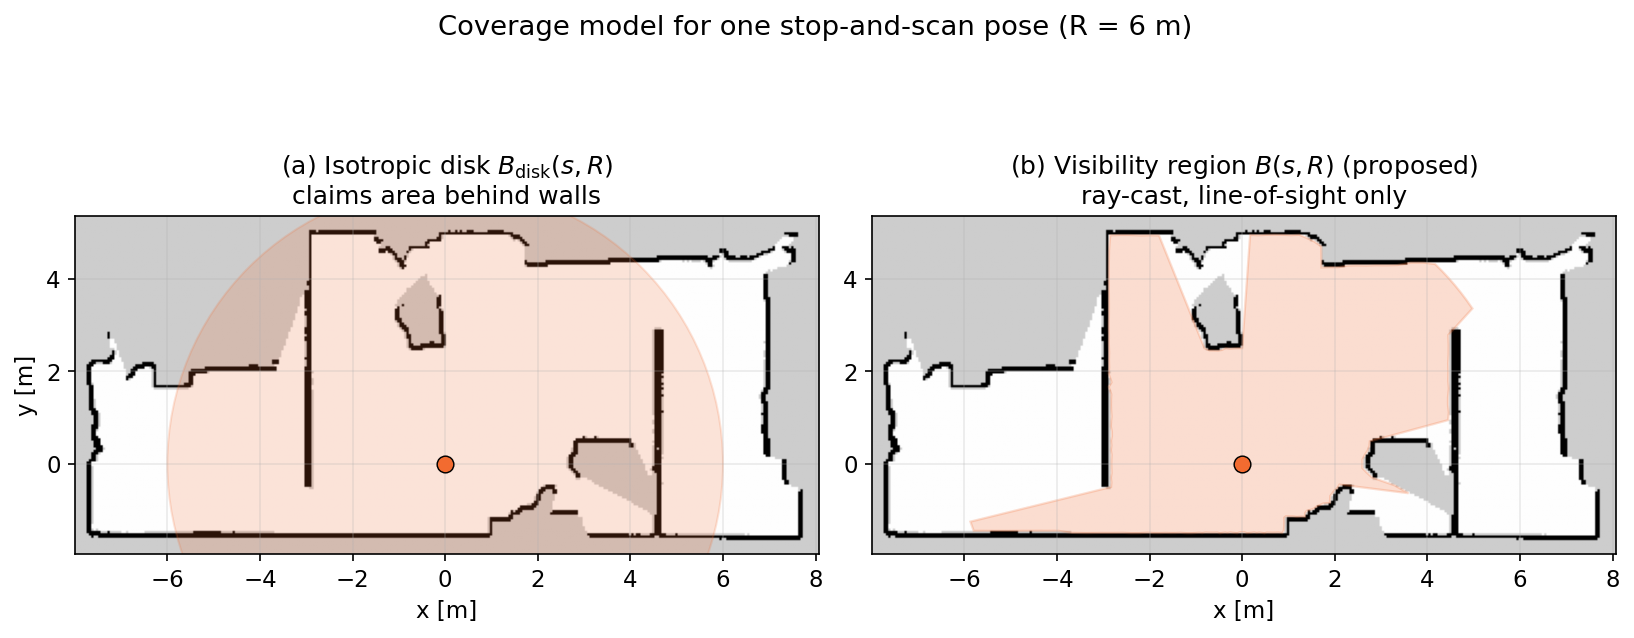
\includegraphics[width=0.85\linewidth]{figures/fig1_concept.png}
\caption{Coverage models for a single scan pose ($R=6$~m).
(\textbf{a})~The isotropic disk $B_{\mathrm{disk}}(s,R)$ counts every free
cell within range as covered, bleeding through walls.
(\textbf{b})~The proposed ray-cast visibility region $B(s,R)$ claims only
genuine line-of-sight area.}
\label{fig:concept}
\end{figure}

\subsection{Ray-Cast Visibility Region (Proposed)}
\label{sec:visibility}

To account for occlusion, we replace the disk with a \emph{ray-cast visibility
region}, a discrete visibility polygon that admits only cells in direct line of
sight of the scan pose. From $s_i$, $K=720$ rays are cast over a full
$360^\circ$ field at uniform angular resolution
$\Delta\theta=360^\circ/K=0.5^\circ$. Each ray is marched outward from $s_i$ in
steps of half a cell and is truncated at the first sample that is either
occupied or unknown; that terminating cell and everything beyond it on the ray
are excluded. Formally, for a free cell $c$ on the ray at azimuth $\theta_k$, let
$\overline{s_i c}$ denote the cells strictly between $s_i$ and $c$ along the ray.
Then

\begin{equation}
B(s_i,R)=\left\{c\in\mathcal{F}:
\lVert c-s_i\rVert \le R \ \wedge\
\mathrm{state}(c')=\textit{free}\ \ \forall\, c'\in\overline{s_i c}\right\}.
\end{equation}

A free cell is claimed as covered only if every intervening cell along the sight
line to it is also mapped free space. The ray stops at the first occupied or
unknown cell: occupied cells ($o\ge\theta_{\mathrm{occ}}$) terminate the ray
because the obstacle blocks the beam, and unknown cells terminate it because the
model refuses to assert visibility through unmapped space. This second condition
is deliberately conservative; the model never ``sees through'' regions the map
cannot vouch for, so $B(s_i,R)$ reports only observation that is geometrically
defensible given the current map. The same stopping rule is applied uniformly
across the model, the implementation, and every experiment in this paper.
Note that the set definition above characterizes the ideal geometric
visibility region and does not depend on the ray discretization; the $K$ rays
and half-cell marching are the implementation that approximates it. At the
range bound the inter-ray arc spacing is $R\,\Delta\theta\approx5.2$~cm for
$R=6$~m, on the order of a single grid cell ($\rho=5$~cm), so the discrete
approximation recovers the ideal region up to single-cell effects at region
boundaries.

By construction $B(s_i,R)\subseteq B_{\mathrm{disk}}(s_i,R)$ for any pose and
range: ray-casting can only remove cells the disk would have claimed, never add
new ones, and the two coincide only for an obstacle-free disk around $s_i$.
Figure~\ref{fig:concept} contrasts the two: where the disk
(Figure~\ref{fig:concept}a) bleeds through partition and perimeter walls, the
visibility region (Figure~\ref{fig:concept}b) is clipped to the genuinely
observable area. Each visibility polygon is computed in pure array operations in
roughly $2$~ms, inexpensive enough to evaluate at every scan candidate online.

\subsection{Line-of-Sight Coverage Metric}
\label{sec:los}

Coverage by a set of scan poses is the union of their visibility regions. For
$S=\{s_1,\dots,s_n\}$ the covered area is

\begin{equation}
C(S)=\bigcup_{i=1}^{n} B(s_i,R),
\end{equation}

and the \emph{line-of-sight (LOS) coverage} is the fraction of mapped free space
observed from at least one scan pose,

\begin{equation}
\mathrm{LOS}(S)=\frac{\lvert C(S)\cap\mathcal{F}\rvert}{\lvert\mathcal{F}\rvert}\in[0,1],
\end{equation}

where $\lvert\cdot\rvert$ counts cells. LOS coverage measures the proportion of
mapped free space for which the sensor set guarantees direct line of sight; the
complement $1-\mathrm{LOS}(S)$ corresponds to mapped free cells that remain
occluded from every scan pose. Because the metric is defined over $\mathcal{F}$
and visibility never propagates through occupied or unknown cells, LOS coverage
is a conservative measure of genuine observation rather than the optimistic
proximity count produced by the disk model. It is the single figure of merit
reported throughout the experiments.

\subsection{Scope: 2D Station Planning for 3D Mapping}
\label{sec:scope2d}

The visibility model and the LOS metric are deliberately two-dimensional: they
reason on the live occupancy grid, a horizontal slice of the environment at the
mapping sensor's height. LOS coverage therefore certifies sight lines to
floor-space cells, not to the full 3D surface set the scanner observes.
Vertical occlusions---shelves, overhanging structures, elevated machinery, or
surfaces stacked at different heights above the same floor cell---are not
represented, and high 2D LOS coverage does not by itself guarantee complete 3D
surface coverage. This scope is a design choice matched to the online setting:
the occupancy grid is what SLAM makes available in real time on the platform;
the 2D visibility polygon is cheap enough to evaluate at every candidate; and
in the room-scale indoor environments targeted here, a pose with unobstructed
2D line of sight to a floor region generally also observes much of the
structure above it, because the scanner acquires a full dome. The contribution
of this paper should accordingly be read as occlusion-aware \emph{2D
scan-station planning for subsequent 3D mapping}; extending the model to a
genuinely 3D visibility representation (voxel-, octree-, or surface-based) is
future work (Section~\ref{sec:discussion}).

\section{Visibility-Based Stop-and-Scan Placement}
\label{sec:placement}

Section~\ref{sec:coverage} defined what a scan pose observes; this section
defines where the robot decides to stop and scan. Because each stationary scan
carries a large fixed cost (minutes per acquisition for the survey-grade
scanner used in our experiments; Section~\ref{sec:setup}), the placement
policy must take as few scans as possible while still guaranteeing LOS coverage
of the free space.

\subsection{Marginal Visibility Gain}

As the robot travels, a scan candidate is raised every $d$ metres of
straight-line displacement in the map frame from the most recent scan pose (net
displacement, not path length, so dwelling or circling in place raises no
candidate). Let $S=\{s_1,\dots,s_m\}$ be the scans accepted so far and
$C(S)=\bigcup_i B(s_i,R)$ their union coverage. The visibility regions of
previously accepted scans are not frozen: at every decision, $C(S)$ is
recomputed on the current occupancy map, so earlier regions expand or contract
as SLAM refines the map (the final reported coverage is evaluated once more on
a single reference map; Section~\ref{sec:setup}). For a candidate pose $p$,
the decision is based on how much \emph{new} line-of-sight area its visibility
region contributes relative to what it sees in total. We define the
\emph{normalized marginal gain}

\begin{equation}
g(p\mid S)=\frac{\lvert B(p,R)\setminus C(S)\rvert}{\lvert B(p,R)\rvert},
\qquad g\in[0,1],
\end{equation}

the fraction of the candidate's own visibility region not already covered, and
the absolute new area

\begin{equation}
a(p\mid S)=\lvert B(p,R)\setminus C(S)\rvert\cdot\rho^2,
\end{equation}

where cells are squares of side $\rho$ (the grid resolution,
$\rho=0.05$~m), so each cell contributes area $\rho^2$ and $a$ is in
m\textsuperscript{2}. Both quantities are defined only for a nonempty
visibility region $B(p,R)$, and are evaluated directly on the visibility
regions of Section~\ref{sec:coverage}, so occlusion is respected: area behind
a wall is never part of $B(p,R)$ and never inflates either the coverage or the
gain. A candidate whose visibility region is degenerate (smaller than
$0.5$~m\textsuperscript{2}, which occurs when the pose projects into an
obstacle or an unmapped pocket where almost every ray is immediately blocked)
is rejected outright before the gain is evaluated, so the denominator of the
normalized gain never vanishes.

\subsection{Dual-Criterion Accept/Skip Rule}

A naive policy would accept a candidate whenever its relative gain exceeds a
threshold, $g\ge\tau$. This single relative test is fragile at the spatial scale
of a room-scale stop-and-scan sensor: because $R$ is comparable to the size of a
room, the region $B(p,R)$ is large, so a small but genuinely occluded pocket contributes
only a tiny \emph{fraction} of that large region and fails the relative test,
even though it is exactly the kind of unscanned area the method exists to
capture. We therefore accept a candidate when \emph{either} a relative \emph{or}
an absolute criterion is met:

\begin{equation}
\textsf{scan}(p)\iff
\big(g(p\mid S)\ge\tau\big)\ \lor\ \big(a(p\mid S)\ge A_{\min}\big),
\end{equation}

and skip it only when both fail. The relative term $\tau$ captures candidates
that open a large new area such as a previously unseen room; the absolute term
$A_{\min}$ rescues small but real occlusion pockets whose new area is a
negligible fraction of the scanner's footprint. Throughout the experiments we
use $\tau=0.30$ and $A_{\min}=5$~m\textsuperscript{2} with range bound
$R=6$~m. Section~\ref{sec:results} shows that coverage and scan count are nearly
flat in $\tau$ over $[0.10,0.50]$, whereas $A_{\min}$ is the operative knob
trading coverage against scan count, with its knee at $5$~m\textsuperscript{2}.

Two disk-based baselines are evaluated against this rule. The first is the
\emph{proximity-spacing rule} of stop-and-go practice: skip any candidate
within $R$ (straight line) of an existing scan. We note explicitly that this
rule is \emph{not} mathematically equivalent to the marginal-gain rule applied
to $B_{\mathrm{disk}}$---a candidate closer than $R$ to an existing scan can
still contribute a crescent of new disk area---so a comparison against it
changes both the coverage model and the acceptance rule. To isolate the
coverage model itself, the ablation of Section~\ref{sec:results} therefore
additionally evaluates a \emph{disk marginal-gain} baseline that applies the
identical dual criterion above with $B_{\mathrm{disk}}$ substituted for $B$
(and disk-based bookkeeping of the covered set); within that pair, the only
difference is the coverage model.

\subsection{Coverage-Completion Phase}

Frontier-driven exploration terminates when the known map stops growing
(Section~\ref{sec:integration}), but convergence of the \emph{map} does not by
itself guarantee that every mapped free cell has been brought into line of
sight: small occluded pockets can remain. The method therefore includes an
optional coverage-completion phase that runs after exploration converges. The
uncovered free cells $\mathcal{F}\setminus C(S)$ are clustered into connected
pockets; for each pocket of area at least $A_{\mathrm{pocket}}$, the robot
navigates into the pocket and takes a stationary scan, repeating until no
qualifying pocket remains. The phase is bounded by per-pocket navigation
timeouts, an overall scan budget, and a list of pockets found unreachable, so it
always terminates. In practice the method does not claim full $100\%$ LOS
coverage: sub-$A_{\mathrm{pocket}}$ fragments at wall and obstacle edges are
reported honestly as residual rather than rounded up.

\subsection{Integration with Exploration}
\label{sec:integration}

The placement policy is embedded in the autonomous exploration loop without
owning the navigation goals. A frontier explorer drives the robot toward
unmapped space on the live occupancy map; a sequencer monitors displacement,
applies the accept/skip rule at each raised candidate, and triggers a stationary
scan when a candidate is accepted, resuming exploration afterward. Completion is
declared by a separate monitor when the count of known cells fails to increase by
a minimum margin over a fixed window while the robot is actively exploring, which
requires no ground truth. Once exploration is complete, the optional
coverage-completion phase runs, after which the run is finalized.

Algorithm~\ref{alg:placement} summarizes the complete placement policy, combining
the marginal-gain evaluation, the dual-criterion accept/skip rule, and the
coverage-completion phase within the exploration loop.

\begin{algorithm}[H]
\caption{Visibility-based stop-and-scan placement}
\label{alg:placement}
\SetAlgoLined
\DontPrintSemicolon
\KwIn{live occupancy map $\mathcal{M}$; range bound $R$; thresholds $\tau$, $A_{\min}$, $A_{\mathrm{pocket}}$; candidate interval $d$}
\KwOut{set of accepted scan poses $S$}
$S \leftarrow \varnothing$;\quad $q \leftarrow$ start pose\;
\While{exploration not converged}{
  drive toward frontier goal on $\mathcal{M}$\;
  \If{$\lVert \mathrm{pose} - q \rVert_2 \ge d$}{
    $p \leftarrow \mathrm{pose}$;\quad $q \leftarrow p$\;
    $B(p,R) \leftarrow \textsc{RayCastVisibility}(\mathcal{M}, p, R)$\;
    \If{$\lvert B(p,R)\rvert \cdot \rho^2 < 0.5$}{
      \textbf{continue} \tcp*{degenerate pose: skip}
    }
    $g \leftarrow \lvert B(p,R)\setminus C(S)\rvert / \lvert B(p,R)\rvert$\;
    $a \leftarrow \lvert B(p,R)\setminus C(S)\rvert \cdot \rho^2$\;
    \If{$g \ge \tau$ \textbf{\emph{or}} $a \ge A_{\min}$}{
      stop and acquire stationary scan at $p$\;
      $S \leftarrow S \cup \{p\}$\;
    }
  }
}
\tcp{Coverage-completion phase (optional)}
\While{$\exists$ pocket $P \subseteq \mathcal{F}\setminus C(S)$ with $\mathrm{area}(P) \ge A_{\mathrm{pocket}}$ and $P$ reachable}{
  navigate into $P$;\quad acquire scan at reached pose $p$\;
  $S \leftarrow S \cup \{p\}$\;
}
\Return{$S$}\;
\end{algorithm}


\section{Experimental Setup}
\label{sec:setup}

\subsection{Platform and Software Stack}

The method is implemented as a set of decoupled ROS~2 nodes. A mobile base
builds a 2D occupancy map online with Cartographer SLAM~\cite{hess2016}; a
frontier explorer~\cite{guler2024} selects goals and drives the robot through
the Nav2 navigation stack~\cite{macenski2020} using a sampling-based
model-predictive path integral (MPPI) controller~\cite{williams2016}; and a
stop-and-scan sequencer applies the
placement policy of Section~\ref{sec:placement}, triggering a stationary scan
whenever a candidate is accepted and gating successive scans so that the long
scan-and-download cycle of the scanner never overlaps with the next acquisition.
All navigation is subject to the platform's physical constraints: Nav2 plans on
an inflated costmap, so every path and every scan candidate keeps the robot
footprint (Figure~\ref{fig:redbot}b) clear of obstacles by the safety margin
of Table~\ref{tab:params} (obstacle dilation radius).
Figure~\ref{fig:arch} shows how these components connect: the frontier
exploration layer proposes and orders navigation goals, and the sequencer
arbitrates the stationary scans, with the ray-cast visibility model of
Section~\ref{sec:coverage} as the component that decides whether each candidate
is scanned or skipped.

\begin{figure}[H]
\centering
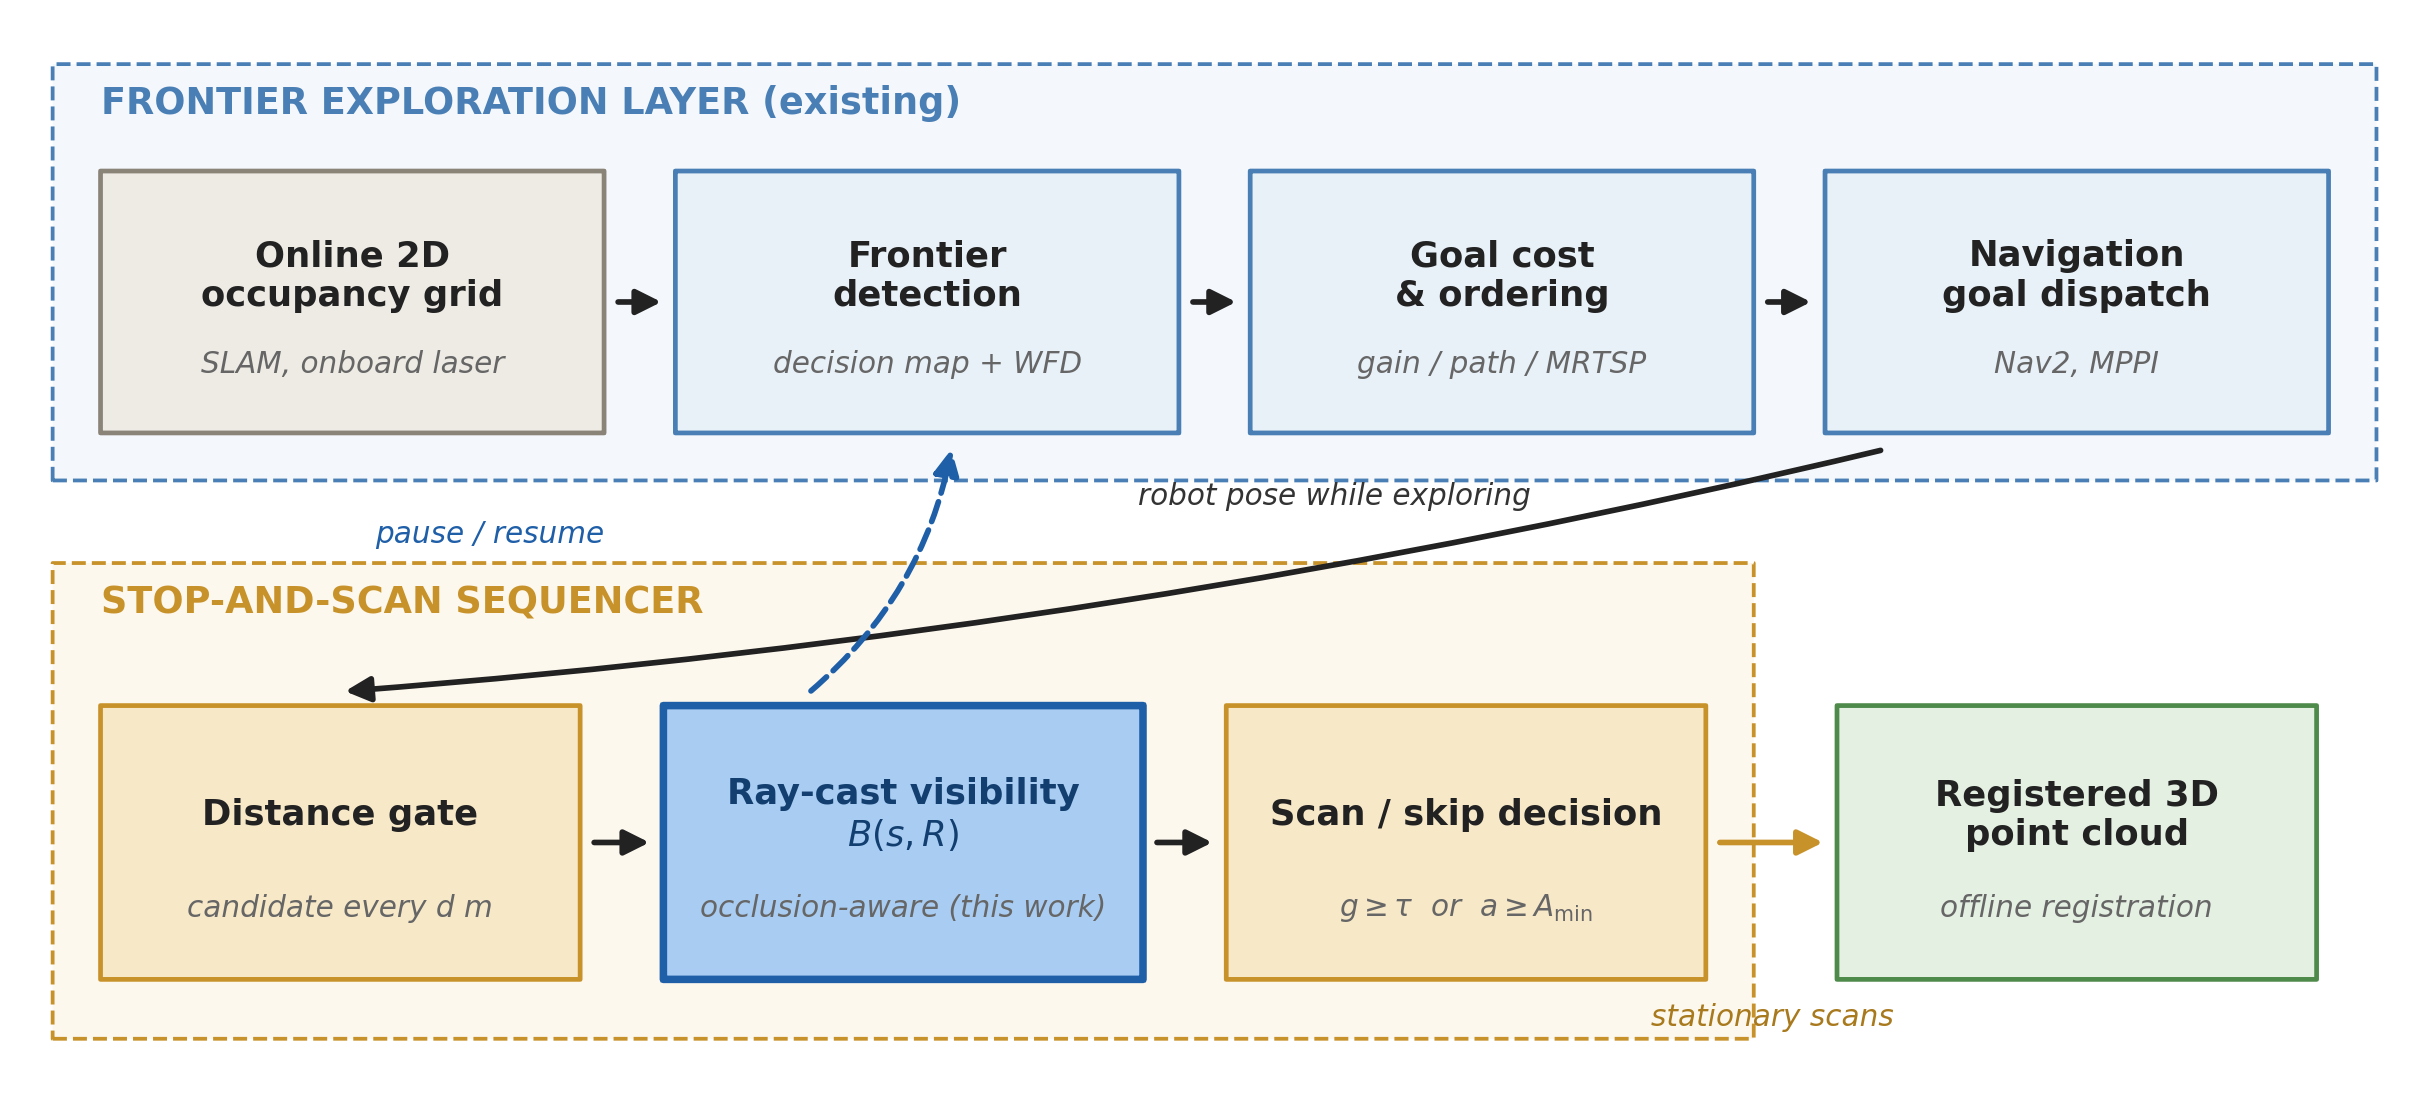
\includegraphics[width=\linewidth]{figures/fig0_architecture.png}
\caption{System architecture. The exploration layer (top) proposes navigation
goals on the live occupancy grid; the stop-and-scan sequencer (bottom) applies
the visibility-based scan/skip rule (highlighted; this work) and triggers
stationary scans that are registered offline.}
\label{fig:arch}
\end{figure}

The target stationary sensor is a Leica BLK360 G1 terrestrial laser scanner. The
software stack includes a driver that connects to a physical BLK360 G1 over WiFi
and executes its colorized-scan workflow, and we verified that the device can be
triggered and read back through this path. The controlled coverage evaluation
(Section~\ref{sec:results}) is conducted \emph{in simulation}: a
TurtleBot3 Waffle is the mobile base in Gazebo~\cite{koenig2004}, and the physical
scanner is replaced by a mock scanner node that reproduces the BLK360
capture-and-download timing and its failure-and-retry behavior. Simulation is used
deliberately for the primary quantitative comparison because it permits a
confound-free, paired ablation in which the disk and visibility rules are replayed
on \emph{identical} maps and candidate paths (Section~\ref{sec:results}), which a
physical run cannot reproduce exactly.

To complement the simulation and validate the workflow on real hardware, we also
built a physical scan platform, RedBOT04, and used it for a fully autonomous
on-hardware disk-versus-visibility comparison in an industrial test room, in
which each skip rule drives live exploration and scan placement and the
deck-mounted BLK360 acquires a stationary scan at every accepted pose
(Section~\ref{sec:fieldsim}); every run's scans were then registered offline as
independent projects (Section~\ref{sec:realhw}). RedBOT04 is a four-wheeled skid-steer mobile base
(footprint $71\times49$~cm) driven by four BLDC gearmotors through an MD200 driver
under RS-485, with an Advantech i7 main controller and an STM32 Nucleo-F746ZG
sub-controller; a YDLiDAR TG30 provides the 2D scan for Cartographer SLAM and Nav2
navigation, and a Leica BLK360 G1 is mounted on the deck as the survey-grade
stationary sensor (Figure~\ref{fig:redbot}). The deck places the scanner's
optical center roughly $0.5$~m above the floor---lower than a typical
$1.5$--$1.8$~m tripod setup---a vantage whose consequences are discussed in
Section~\ref{sec:discussion}.

\begin{figure}[H]
\centering
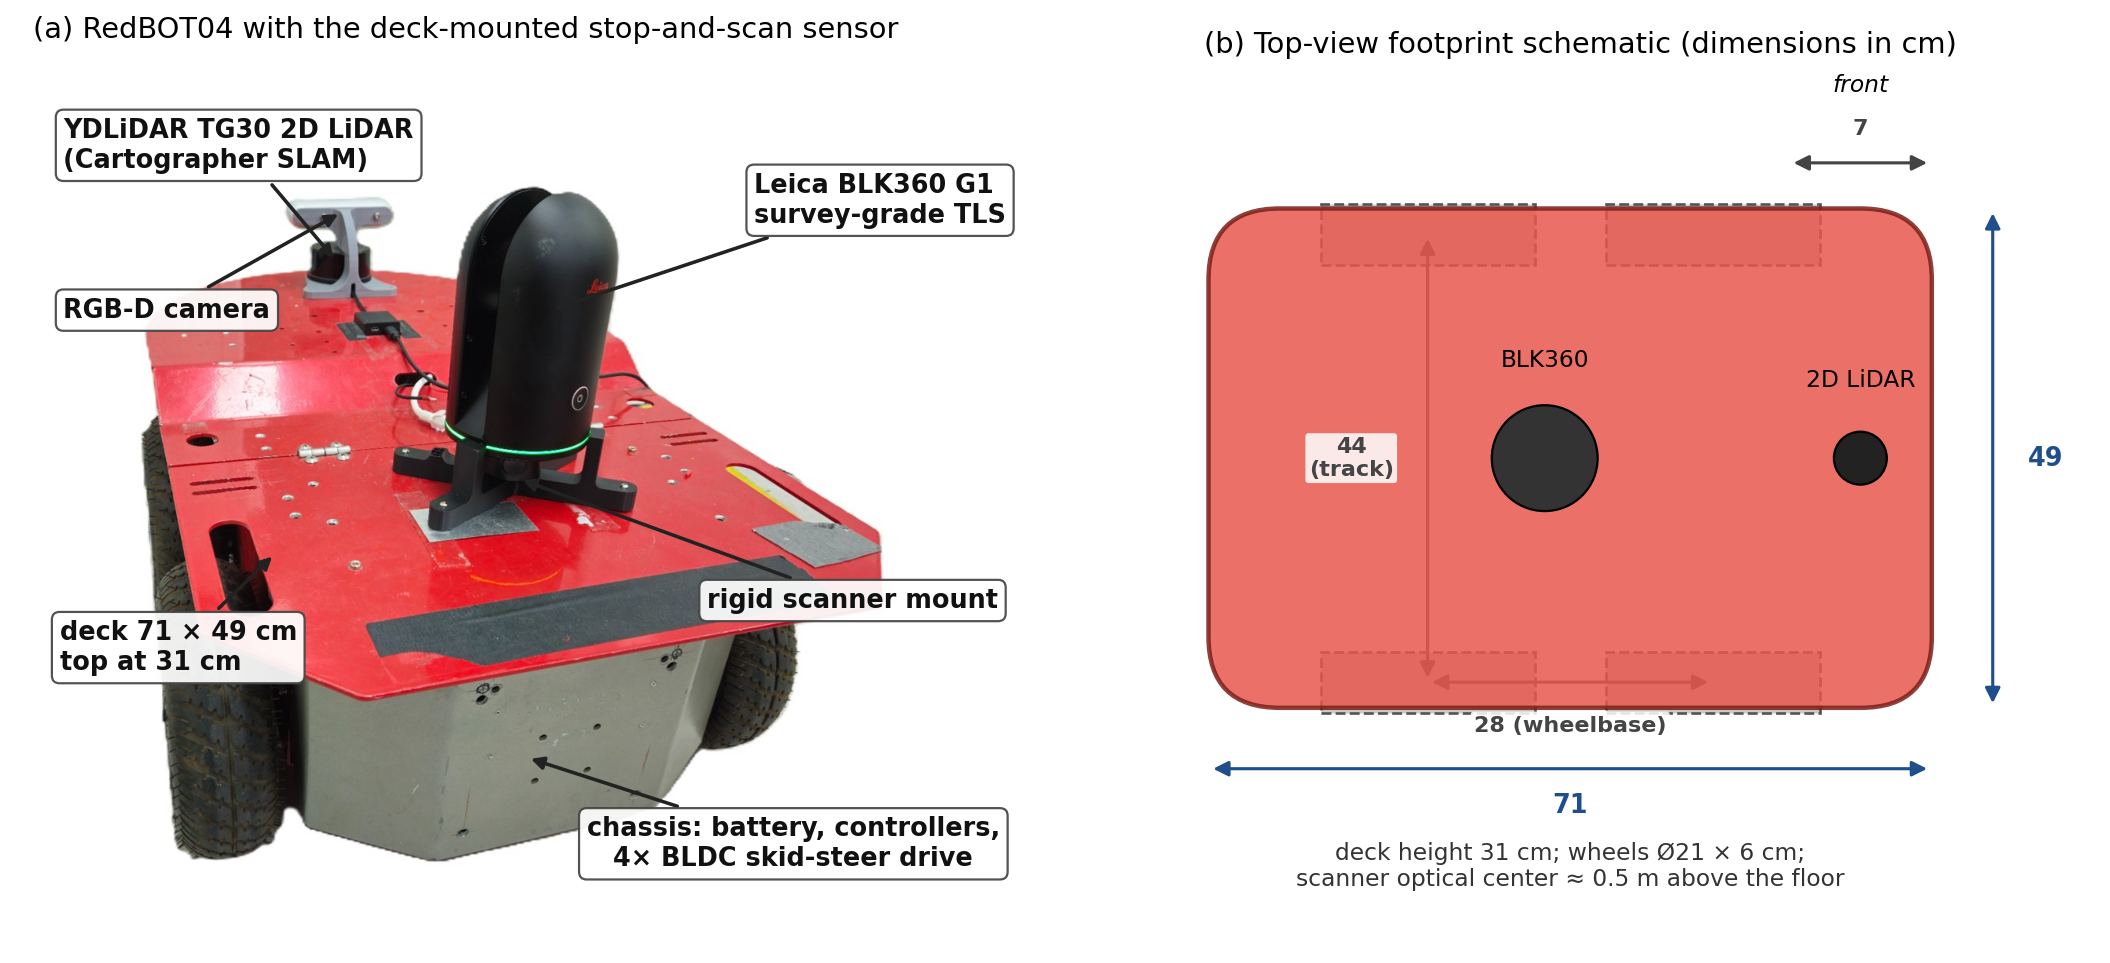
\includegraphics[width=\linewidth]{figures/fig9_redbot04_platform_annot.png}
\caption{RedBOT04 mobile scan platform. (\textbf{a})~Annotated view with the
deck-mounted Leica BLK360 G1; (\textbf{b})~top-view footprint schematic with
the principal dimensions (cm).}
\label{fig:redbot}
\end{figure}

\subsection{Environments and Metric}

Two indoor worlds are used. The single-room world is generated from a real
BLK360 \texttt{.e57} scan of a laboratory space, converted to a 2D occupancy
grid and then to a Gazebo world, so the simulated geometry reflects a real
environment. The multi-room world extends this with two interior partitions and
offset doorways, producing three rooms with mutual occlusion; it is the setting
in which the difference between Euclidean-disk and line-of-sight coverage is most
pronounced. For the real-hardware experiments (Sections~\ref{sec:fieldsim}
and~\ref{sec:realhw}), a physical industrial test room is used. It is an open
exhibition and staging space with a flat, reflective floor; a display wall of
monitors and product panels runs along one side, and freestanding equipment
cases and furniture create genuine self-occlusion. Floor markings indicate the
survey reference layout. The room is representative of the factory and
demonstration environments the platform targets, and it is shown in
Figure~\ref{fig:testroom}. Its mapped free space spans approximately
$16\times8.5$~m, about $105$~m\textsuperscript{2} of free floor area on the
reference map.
The figure of merit is LOS coverage (Section~\ref{sec:los}). Because
each autonomous run maps a slightly different extent of free space, for any
cross-run comparison we re-evaluate every run on a single common reference map
(the most complete map among the runs being compared) so that all runs share the
same free-space denominator. Scan count is reported alongside coverage as the
cost term. Unless noted, experiments use $R=6$~m, $\tau=0.30$,
$A_{\min}=5$~m\textsuperscript{2}, a candidate every $d=3$~m of net displacement,
and $K=720$ rays. Table~\ref{tab:params} lists the full parameter set.

\begin{figure}[H]
\centering
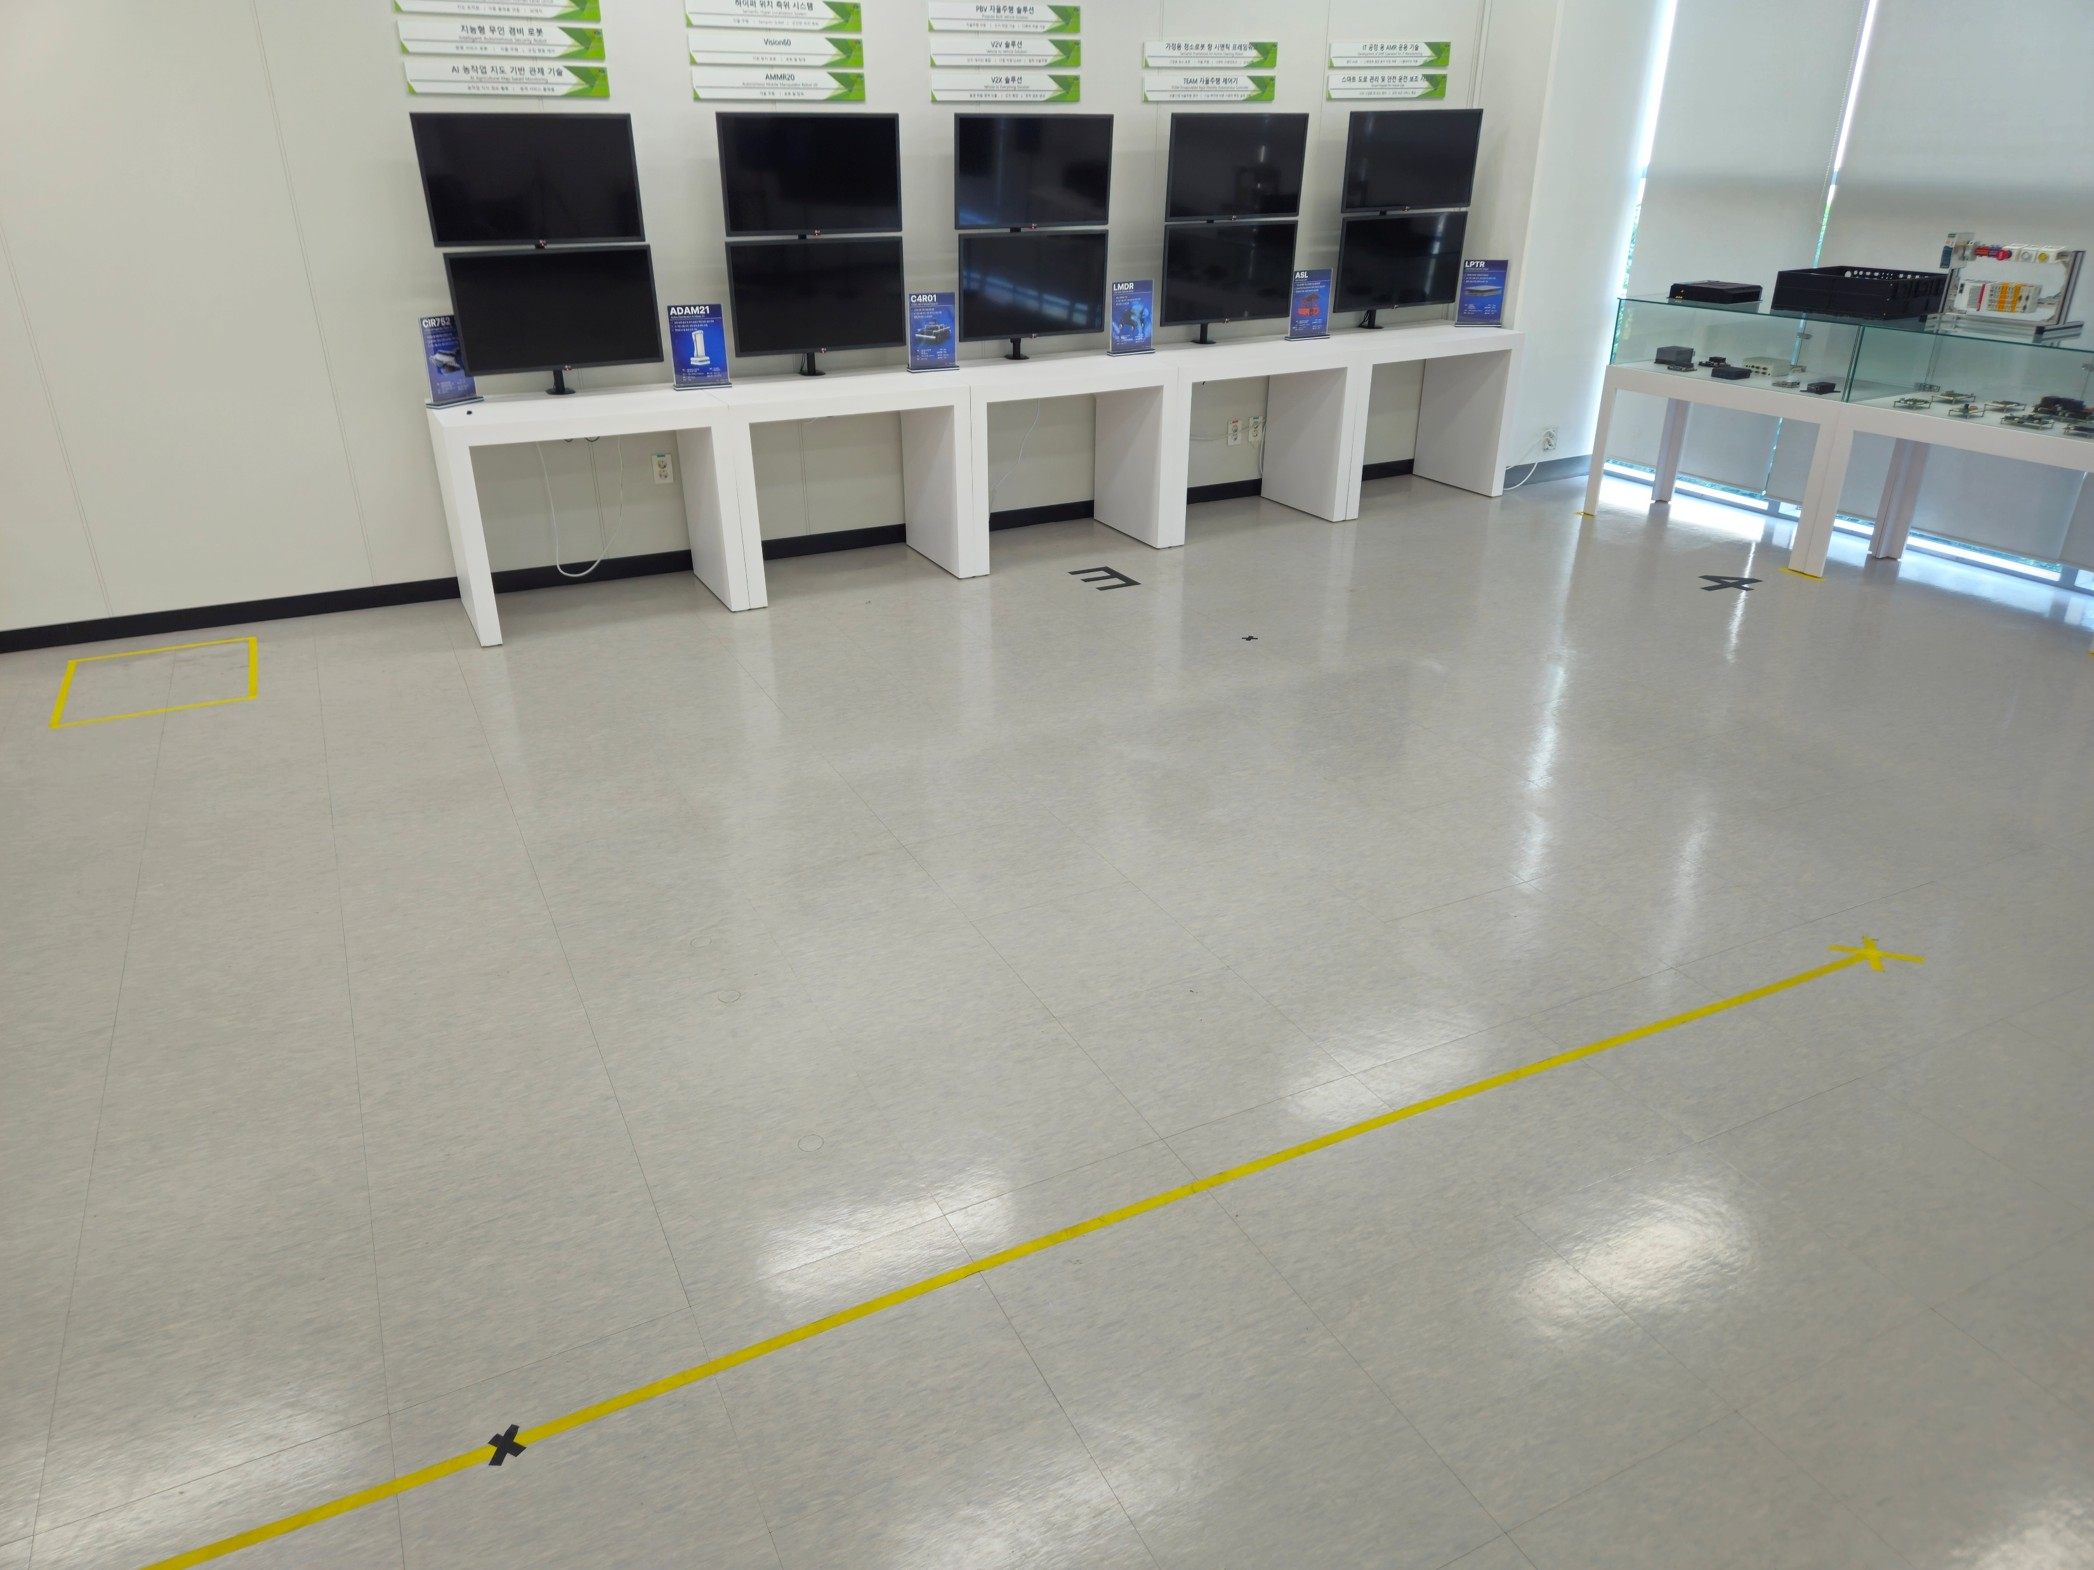
\includegraphics[width=0.9\linewidth]{figures/fig10_testroom.jpg}
\caption{Physical industrial test room used for the real-hardware experiments
(Sections~\ref{sec:fieldsim} and~\ref{sec:realhw}).}
\label{fig:testroom}
\end{figure}

\begin{table}[H]
\caption{Principal parameters of the stop-and-scan mapping subsystem. Values in
the upper block are the operating point used in all experiments unless otherwise
noted; values in the lower block are tuned per environment.}
\label{tab:params}
\newcolumntype{P}{>{\raggedright\arraybackslash}X}
\begin{tabularx}{\linewidth}{l l P}
\toprule
\textbf{Parameter} & \textbf{Value} & \textbf{Description} \\
\midrule
Range bound $R$              & 6~m   & Maximum distance out to which the visibility region $B(s,R)$ is evaluated. \\
Relative threshold $\tau$    & 0.30  & Minimum fraction of new visible area for the relative accept criterion. \\
Absolute threshold $A_{\min}$& 5~m\textsuperscript{2} & Minimum new visible area for the absolute accept criterion. \\
Candidate interval $d$       & 3~m   & Net straight-line displacement between successive scan candidates. \\
Ray count $K$                & 720   & Number of rays per visibility computation ($\Delta\theta=0.5^\circ$). \\
Free threshold $\theta_{\mathrm{free}}$ & 25 & Upper occupancy value for a cell to count as mapped free space. \\
Occupied threshold $\theta_{\mathrm{occ}}$ & 65 & Lower occupancy value for a cell to terminate a ray as an obstacle. \\
Degenerate cut               & 0.5~m\textsuperscript{2} & Minimum visibility-region area; smaller candidates are rejected. \\
\midrule
Scan-and-download time       & env.-tuned & Mock-scanner capture-plus-download duration matching the BLK360 G1 cycle. \\
Bilateral-filter std.\ dev.  & env.-tuned & Spatial and range Gaussian kernel widths for decision-map construction. \\
Obstacle dilation radius     & env.-tuned & Morphological dilation enforcing a safety clearance margin. \\
Minimum frontier size        & env.-tuned & Frontier clusters smaller than this are discarded as noise. \\
Completion pocket area $A_{\mathrm{pocket}}$ & env.-tuned & Minimum uncovered-pocket area triggering a completion scan. \\
\bottomrule
\end{tabularx}
\end{table}

\section{Results}
\label{sec:results}

We evaluate the visibility-based policy on two axes, LOS coverage and
stationary scan count, organizing the evaluation so that the most rigorous
evidence carries the argument. Four placement policies are compared throughout:
(i)~a \emph{uniform no-skip} reference that scans at every candidate---the
fixed-interval policy of stop-and-go practice and an upper reference on the
coverage attainable along a path; (ii)~the \emph{disk spacing} baseline, the
proximity rule of stop-and-go practice; (iii)~the \emph{disk marginal-gain}
baseline, which applies the identical accept/skip rule as our policy to the
disk coverage model (Section~\ref{sec:placement}); and (iv)~the proposed
\emph{ray-cast visibility} policy. The disk baselines represent the de facto
online coverage treatment in stop-and-go practice
(Section~\ref{sec:related}); published TLS scan-planning methods are not
applicable as online baselines because they optimize viewpoints offline over a
prior environment model~\cite{tls-scanplanning,dehbi2021,knechtel2025},
whereas the regime studied here requires every decision to be made on the live
map of an unknown environment. The simulation study comes first;
Section~\ref{sec:fieldsim} then reports a fully autonomous on-hardware
disk-versus-visibility comparison in a physical industrial test room, with
scans acquired live, and Section~\ref{sec:realhw} closes the loop by
registering every run's scans offline, run by run.

\subsection{Coverage Model and Single-Room Placement}

Figure~\ref{fig:concept} contrasts the two coverage models for a single scan
pose: the disk claims area on the far side of partition and perimeter walls,
whereas the ray-cast visibility region is clipped to genuine line of sight. On
the full single-room world, the visibility stop-and-scan policy places four
scans and reaches $97.9\%$ LOS coverage (Figure~\ref{fig:singleroom}). Varying
the range bound $R\in\{5,6,10\}$~m yields $97$--$98\%$ LOS in all cases
(Figure~\ref{fig:rsweep}); larger $R$ needs fewer scans but spreads them apart,
reducing inter-scan overlap. We adopt $R=6$~m for three reasons: it balances
coverage against the scan-to-scan overlap that downstream point-cloud
registration benefits from; it keeps every cell claimed as covered well inside
the scanner's highest-accuracy band, since the BLK360 G1 specifies a 3D point
accuracy of $6$~mm at $10$~m ($8$~mm at $20$~m)~\cite{leica-blk360}; and it
matches the room-scale dimensions of the indoor environments targeted here,
which are rarely much larger than $6$~m across.

\begin{figure}[H]
\centering
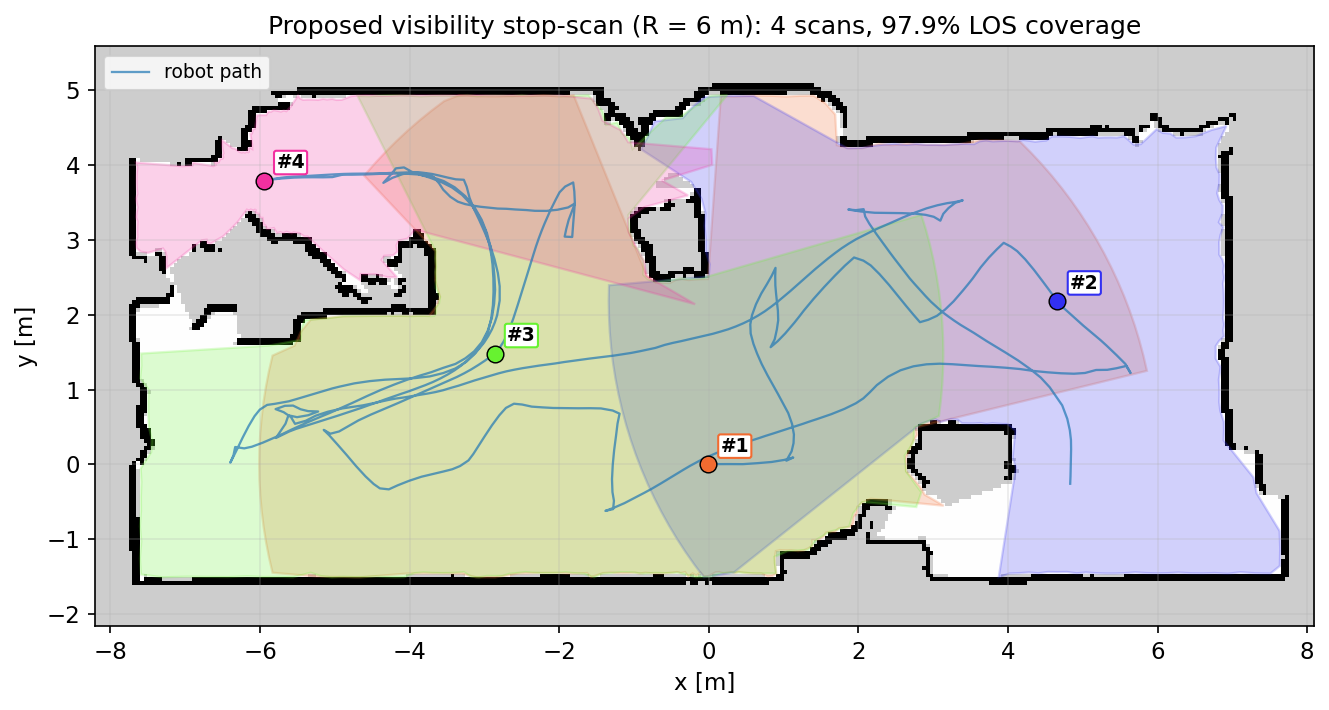
\includegraphics[width=0.7\linewidth]{figures/fig2_singleroom_sota.png}
\caption{Proposed visibility stop-and-scan on the single-room world
($R=6$~m): 4~scans, $97.9\%$ LOS coverage. Each accepted scan pose (marker)
and its visibility polygon share one color, indexed by scan order
($\#1\dots\#4$); the grayscale background is the occupancy map (light gray
free, black occupied, darker gray unknown) and the blue line is the robot
path. The same color convention is used in all placement figures.}
\label{fig:singleroom}
\end{figure}

\begin{figure}[H]
\centering
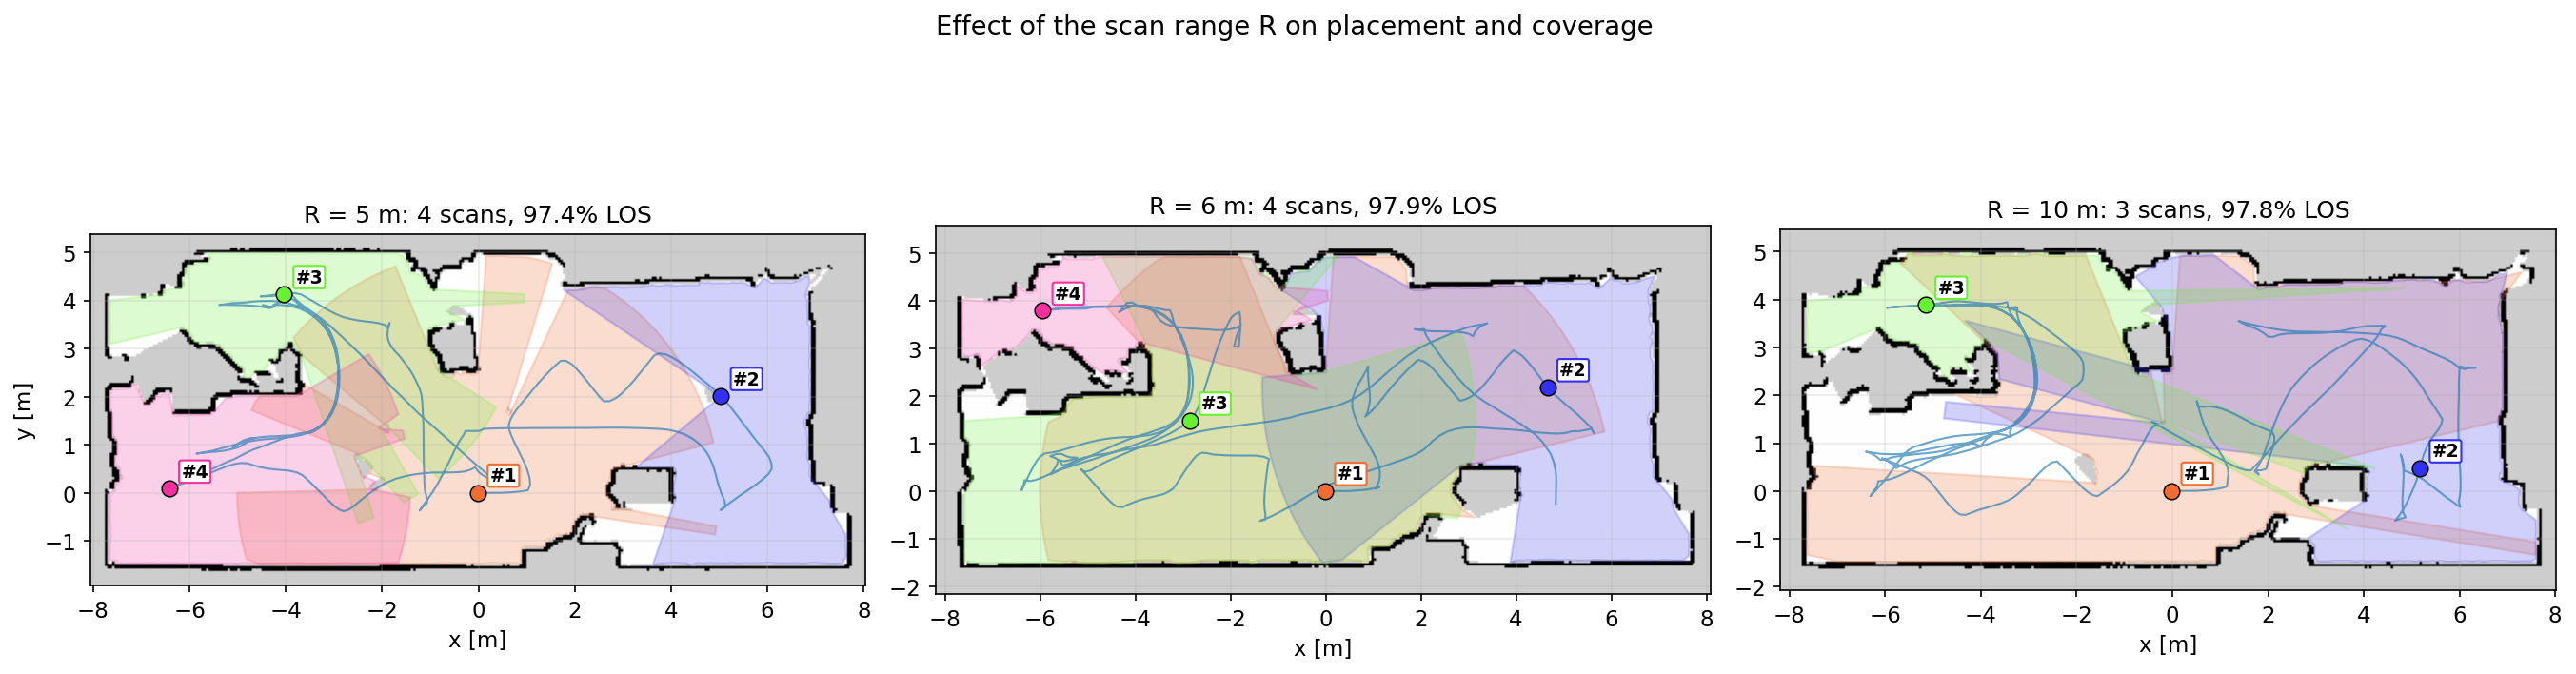
\includegraphics[width=0.95\linewidth]{figures/fig3_R_sweep.png}
\caption{Effect of the range bound $R$ on placement and coverage for
$R=5/6/10$~m. Larger $R$ needs fewer scans but spreads them; $R=6$~m balances
coverage ($97.9\%$) against inter-scan overlap for registration.}
\label{fig:rsweep}
\end{figure}

\subsection{Controlled Skip-Rule Ablation (Primary Result)}

The decisive comparison isolates the only variable of interest, the accept/skip
decision, from the stochasticity of autonomous exploration. On a fixed
environment map and a fixed candidate sequence (a logged trajectory sampled every
$2$~m of path length), we replay \emph{both} skip rules, so the disk and
visibility policies see identical maps and identical candidate poses and differ
only in which candidates they accept (Figure~\ref{fig:ablation}). This
deterministic, paired design removes the confound that, in live runs, which
rooms get mapped is dominated by navigation through narrow doorways rather than
by the skip rule.

Across $N=5$ single-room and $N=10$ multi-room trajectories (five per coverage
model), the visibility rule raises LOS coverage from $77.0\pm4.9\%$ to
$85.4\pm6.2\%$ in the single-room world and from $77.0\pm6.4\%$ to $84.0\pm9.2\%$
in the three-room world, at a cost of one to two additional scans on average
(single-room $2.0\pm0.0\to3.6\pm0.9$; multi-room $2.3\pm0.5\to3.6\pm0.7$); see
Figure~\ref{fig:summary} and Table~\ref{tab:ablation}. To bound what is
attainable along these paths, we also replay a uniform no-skip policy that scans
at every candidate: it reaches $91.9\pm7.0\%$ LOS (single-room) and
$86.6\pm9.9\%$ (multi-room), but at $28.0$ and $40.8$ scans on average. The
visibility rule thus comes within $6.5$ and $2.6$ percentage points of this
brute-force upper reference while taking roughly an eighth as many scans,
and exceeds the disk baseline by $+8.4$ and $+7.0$ percentage points for one to
two additional scans. On paths that traverse
every room, where the disk rule's blindness to occlusion is fully exercised, the
per-path coverage gain reaches $+21$ to $+23$ percentage points. The disk
spacing rule is structurally capped: once two scans are placed, almost every
later candidate lies within $R$ (straight line) of a prior scan, so it stops
scanning even though walls occlude much of the area it counts as covered.

The disk marginal-gain baseline isolates the coverage model from the
acceptance rule. Under the identical dual criterion of
Section~\ref{sec:placement}, the disk model accepts $2.6\pm0.5$ scans for
$77.7\pm3.8\%$ LOS in the single-room world---essentially the spacing rule's
result---and $2.9\pm0.3$ scans for only $59.1\pm1.3\%$ LOS in the multi-room
world, markedly \emph{worse} than even the spacing rule. The mechanism is
instructive. Because $B_{\mathrm{disk}}$ claims area through partitions, the
disk model's own coverage bookkeeping saturates after the first few
acceptances: every later candidate appears almost fully covered, so the rule
stops scanning while whole rooms remain unobserved. The spacing rule, blind to
coverage altogether, at least keeps accepting whenever the robot moves $R$
away from all prior scans and thus occasionally scans another room by
accident. That the same acceptance rule produces a $24.9$-point LOS gap
between the two coverage models in the multi-room world ($59.1\%$ versus
$84.0\%$) is the sharpest form of this paper's claim: the deficiency lies in
the disk coverage model itself, not in the acceptance rule attached to it.

\begin{figure}[H]
\centering
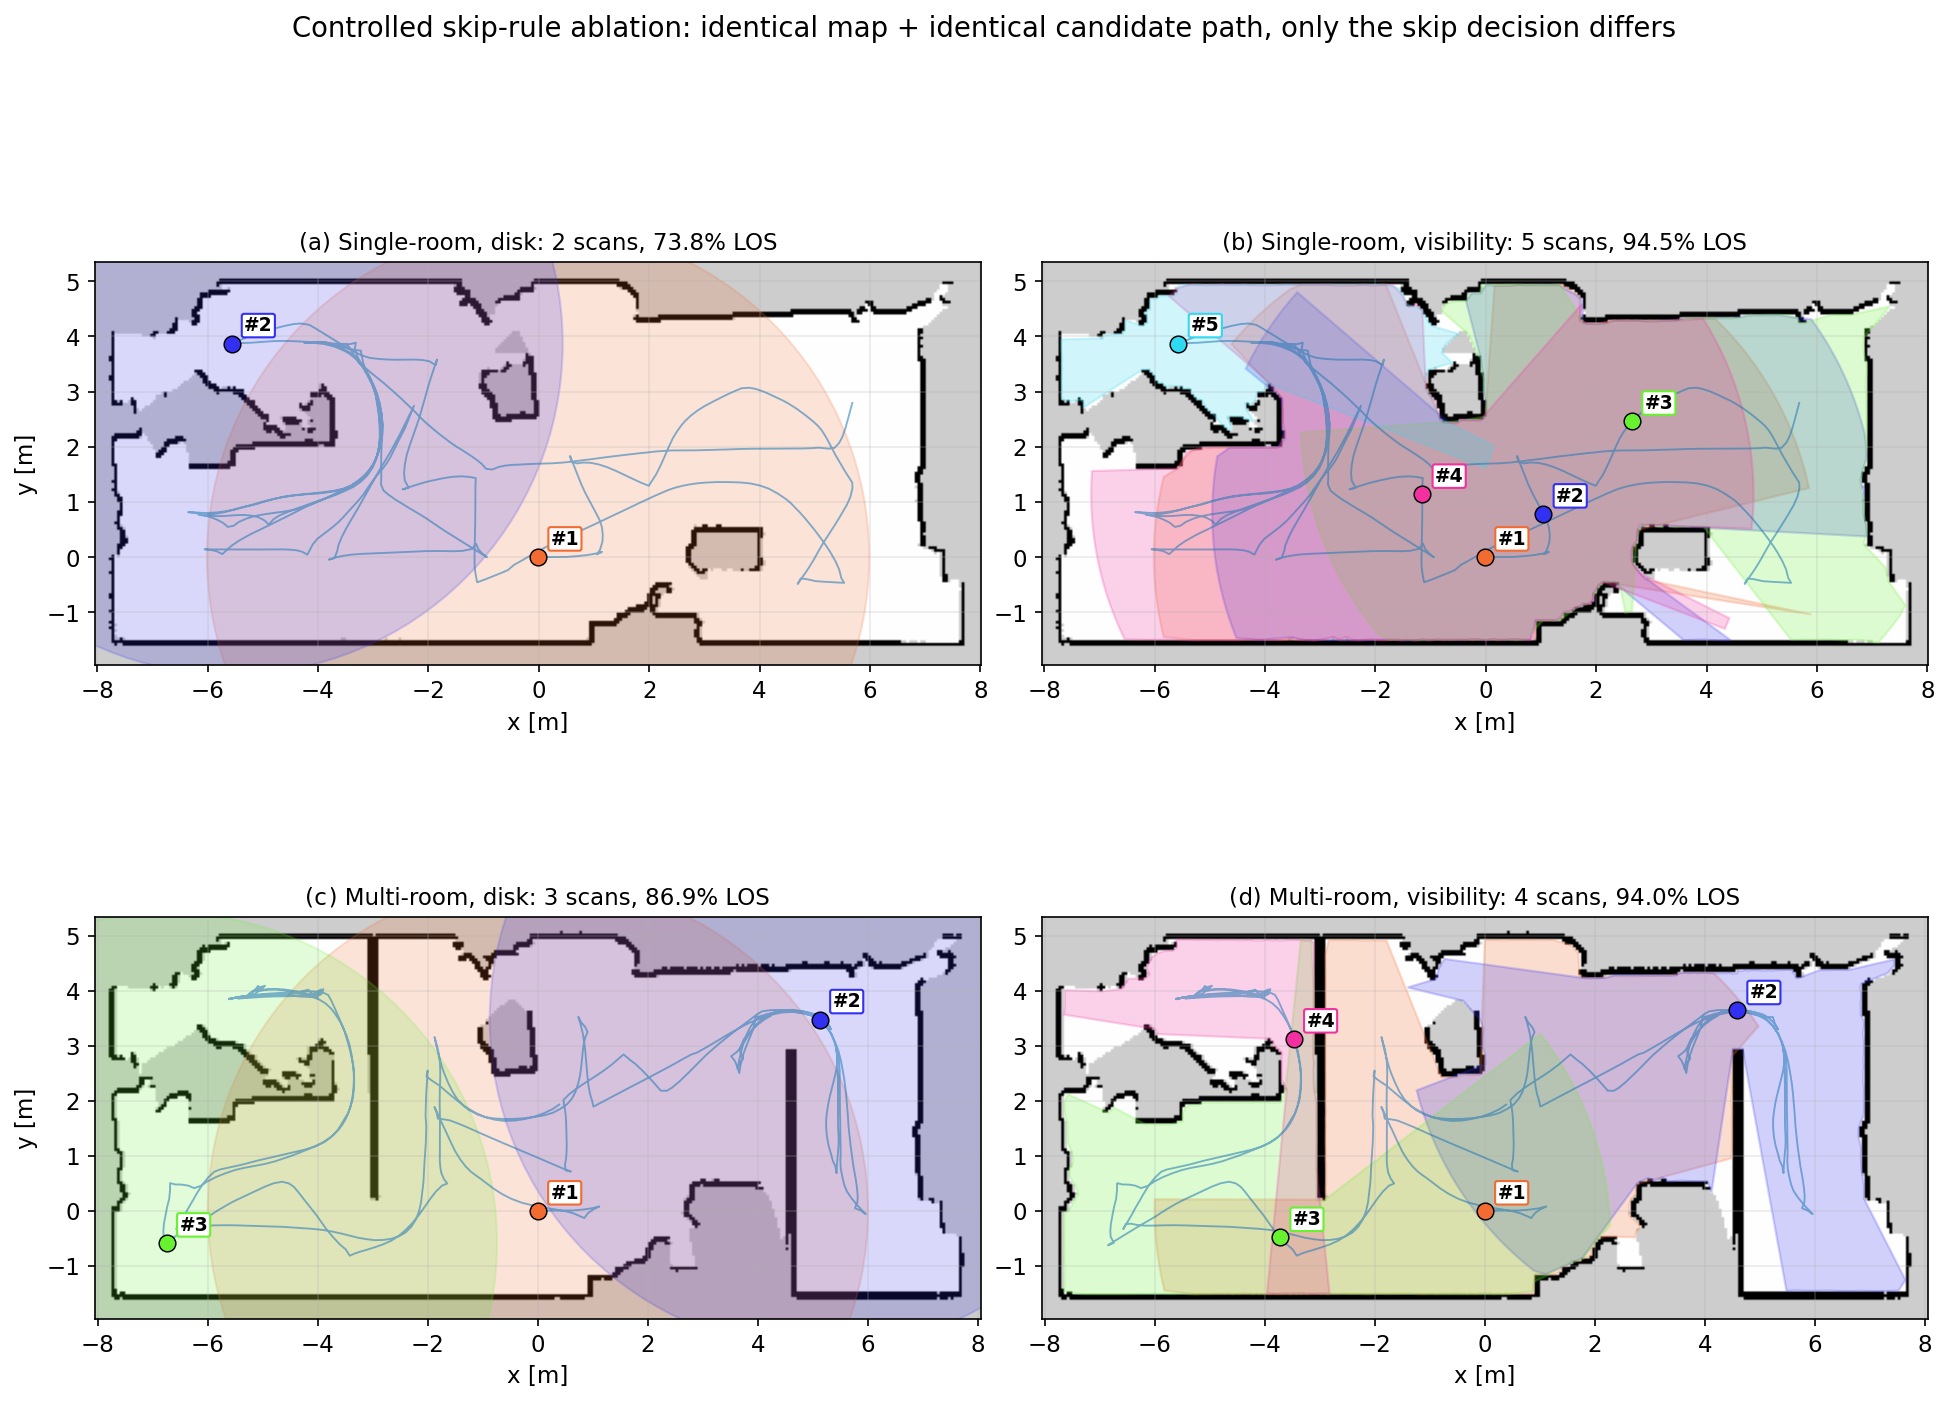
\includegraphics[width=0.95\linewidth]{figures/fig5_skip_ablation.png}
\caption{Controlled skip-rule ablation on an identical map and candidate
path; only the skip decision differs. (\textbf{a},\textbf{b})~Single-room and
(\textbf{c},\textbf{d})~multi-room, under the disk spacing rule
(\textbf{a},\textbf{c}) and the visibility rule (\textbf{b},\textbf{d}).}
\label{fig:ablation}
\end{figure}

\begin{figure}[H]
\centering
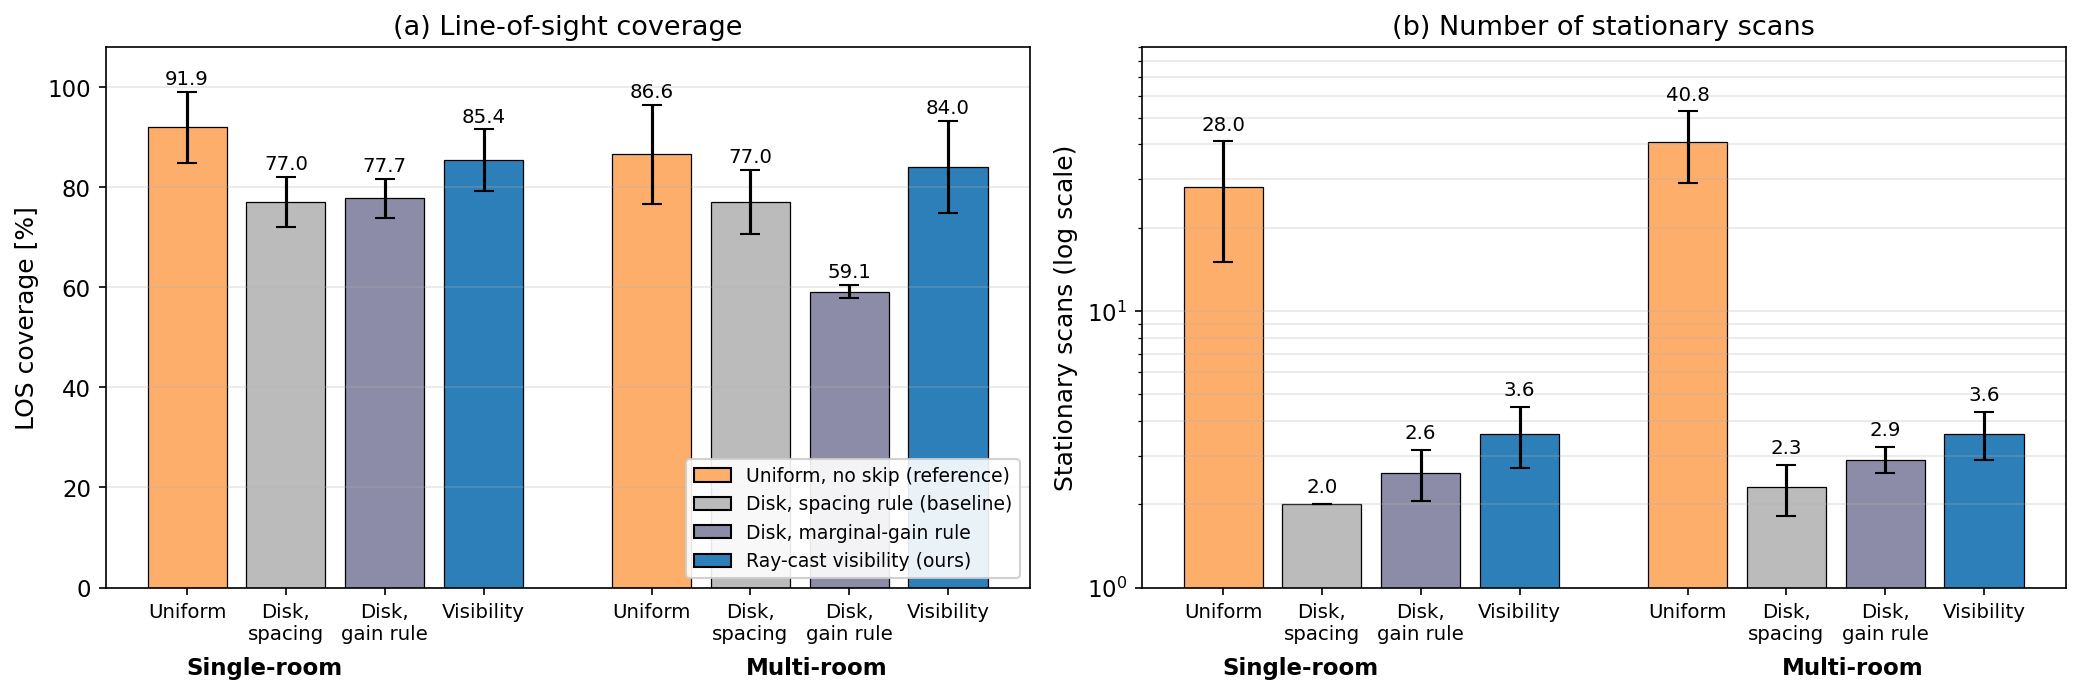
\includegraphics[width=0.95\linewidth]{figures/fig7_summary.png}
\caption{Four-way skip-rule comparison on identical paths ($N=5$ single-room
and $N=10$ multi-room trajectories, paired per path). (\textbf{a})~LOS
coverage; (\textbf{b})~stationary scan count, log scale
(mean\,$\pm$\,s.d.).}
\label{fig:summary}
\end{figure}

\begin{table}[H]
\caption{Controlled skip-rule ablation: four placement policies replayed on
the same fixed candidate sequences ($N=5$ single-room paths; $N=10$ multi-room
paths). Values are mean\,$\pm$\,s.d. The uniform no-skip policy is an upper
reference on the LOS attainable along the path, at a prohibitive scan count;
the disk marginal-gain row applies the identical accept/skip rule as the
visibility policy, so within each environment that pair differs only in the
coverage model.}
\label{tab:ablation}
\newcolumntype{Z}{>{\centering\arraybackslash}X}
\begin{tabularx}{\linewidth}{l l Z Z}
\toprule
\textbf{Environment} & \textbf{Coverage model} & \textbf{LOS coverage (\%)} & \textbf{Scans} \\
\midrule
\multirow{4}{*}{Single-room} & Uniform, no skip (reference) & $91.9\pm7.0$ & $28.0\pm13.0$ \\
                             & Disk, spacing rule (baseline) & $77.0\pm4.9$ & $2.0\pm0.0$ \\
                             & Disk, marginal-gain rule      & $77.7\pm3.8$ & $2.6\pm0.5$ \\
                             & Ray-cast visibility (ours)   & $\mathbf{85.4\pm6.2}$ & $3.6\pm0.9$ \\
\midrule
\multirow{4}{*}{Multi-room}  & Uniform, no skip (reference) & $86.6\pm9.9$ & $40.8\pm11.8$ \\
                             & Disk, spacing rule (baseline) & $77.0\pm6.4$ & $2.3\pm0.5$ \\
                             & Disk, marginal-gain rule      & $59.1\pm1.3$ & $2.9\pm0.3$ \\
                             & Ray-cast visibility (ours)   & $\mathbf{84.0\pm9.2}$ & $3.6\pm0.7$ \\
\bottomrule
\end{tabularx}
\noindent\footnotesize{On paths that traverse every room, the per-path gain
of the visibility rule over the disk spacing rule reaches $+21$ to $+23$
percentage points; the means above are over all paths including
partial-traversal paths. All policies traverse the identical candidate path,
so total travel distance is the same across rows; the policies differ only in
scan count, the dominant cost in stop-and-scan sensing.}
\end{table}

\subsection{Live Multi-Room Demonstration (Qualitative)}

Figure~\ref{fig:multiroom} shows a single live autonomous run on the multi-room
world under each coverage model. The disk policy stops after two scans at
$46.9\%$ LOS, having counted an entire room behind a partition as covered through
the wall; the visibility policy places one scan per room, three in total, and
reaches $95.1\%$ LOS. We present this run as a qualitative demonstration rather
than a statistical result: in live runs on the partitioned world, which rooms get
mapped (a function of frontier selection and navigation through narrow, offset
doorways) varies from run to run and dominates the measured coverage largely
independently of the skip rule, which inflates variance and shrinks the apparent
gap. The rigorous, confound-free claim is therefore the controlled ablation
above; the live run illustrates how that difference manifests in a complete
mission.

\begin{figure}[H]
\centering
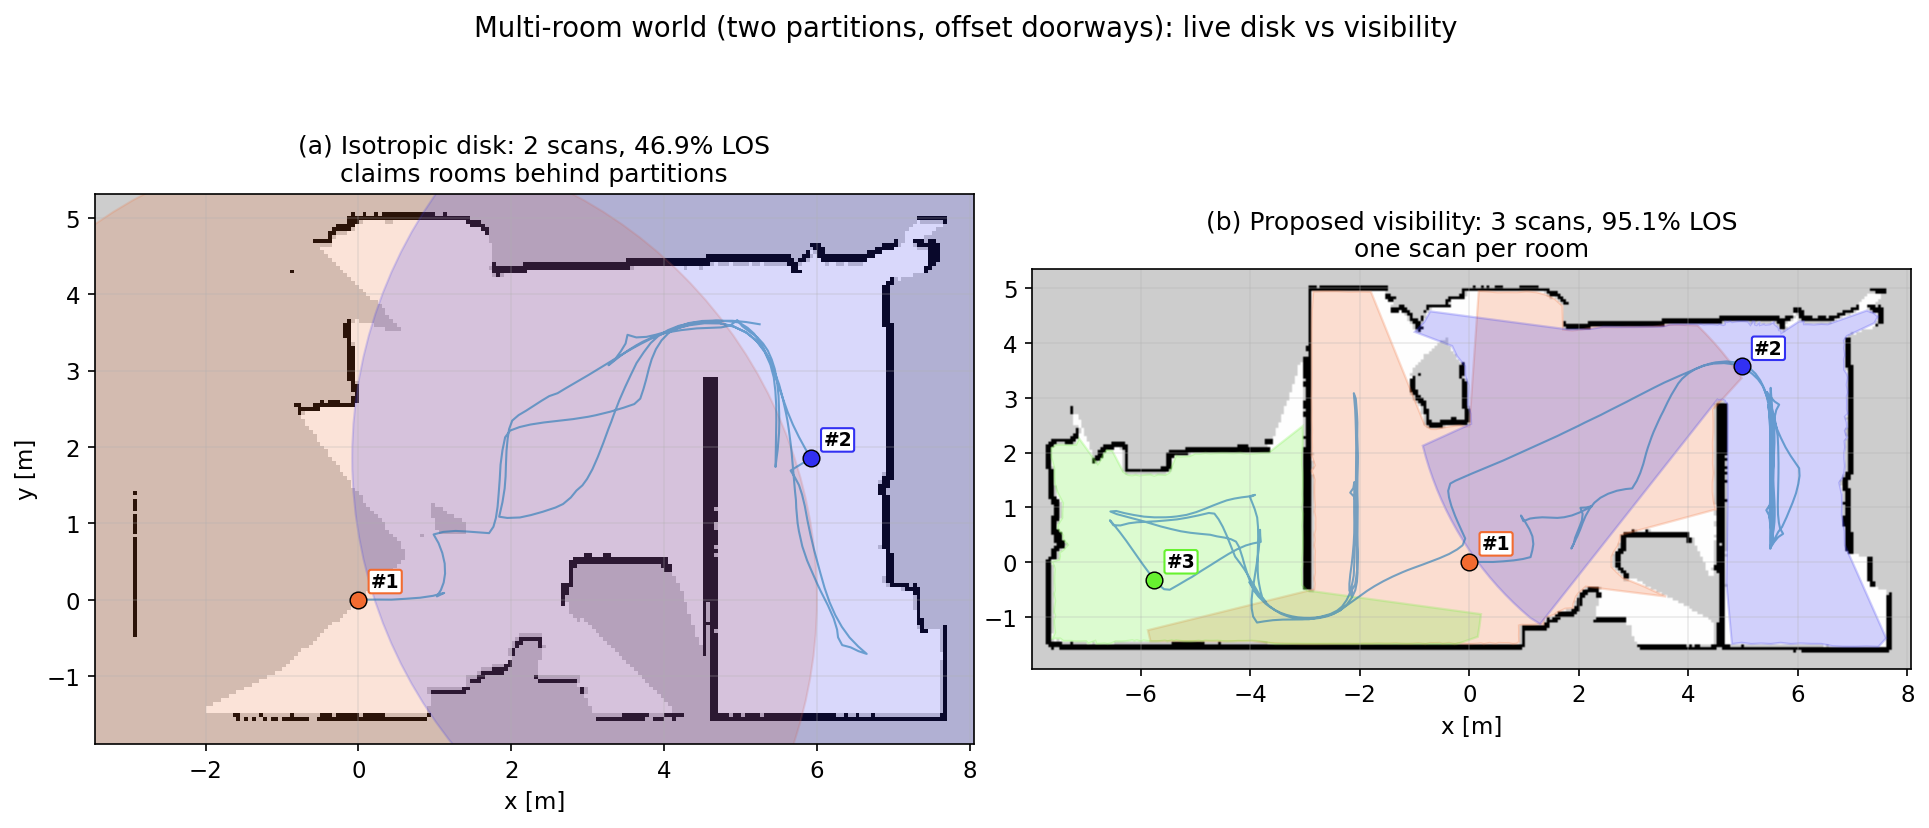
\includegraphics[width=0.95\linewidth]{figures/fig4_multiroom_compare.png}
\caption{Multi-room world (two partitions, offset doorways): live disk vs.\
visibility. (\textbf{a})~The disk model skips candidates within $R$ of a prior
scan through the partitions, giving 2~scans and $46.9\%$ LOS with a whole room
unscanned. (\textbf{b})~The visibility model scans once per room, giving 3~scans
and $95.1\%$ LOS.}
\label{fig:multiroom}
\end{figure}

\subsection{Coverage Completion}

With the coverage-completion phase enabled, the robot continues after frontier
convergence to drive into and scan the remaining uncovered pockets. Over $N=5$
runs this raises LOS coverage to $98.9\pm0.9\%$ using $5.0\pm1.2$ total scans on
average ($3.2$ frontier plus $1.8$ completion scans), with no unreachable pockets
across the five runs. A representative run reaches $99.6\%$ LOS with three
frontier scans followed by three completion scans (Figure~\ref{fig:completion}).
The method does not claim a full $100\%$: residual fragments smaller than the
minimum pocket area at wall and obstacle edges are reported as remaining.

\begin{figure}[H]
\centering
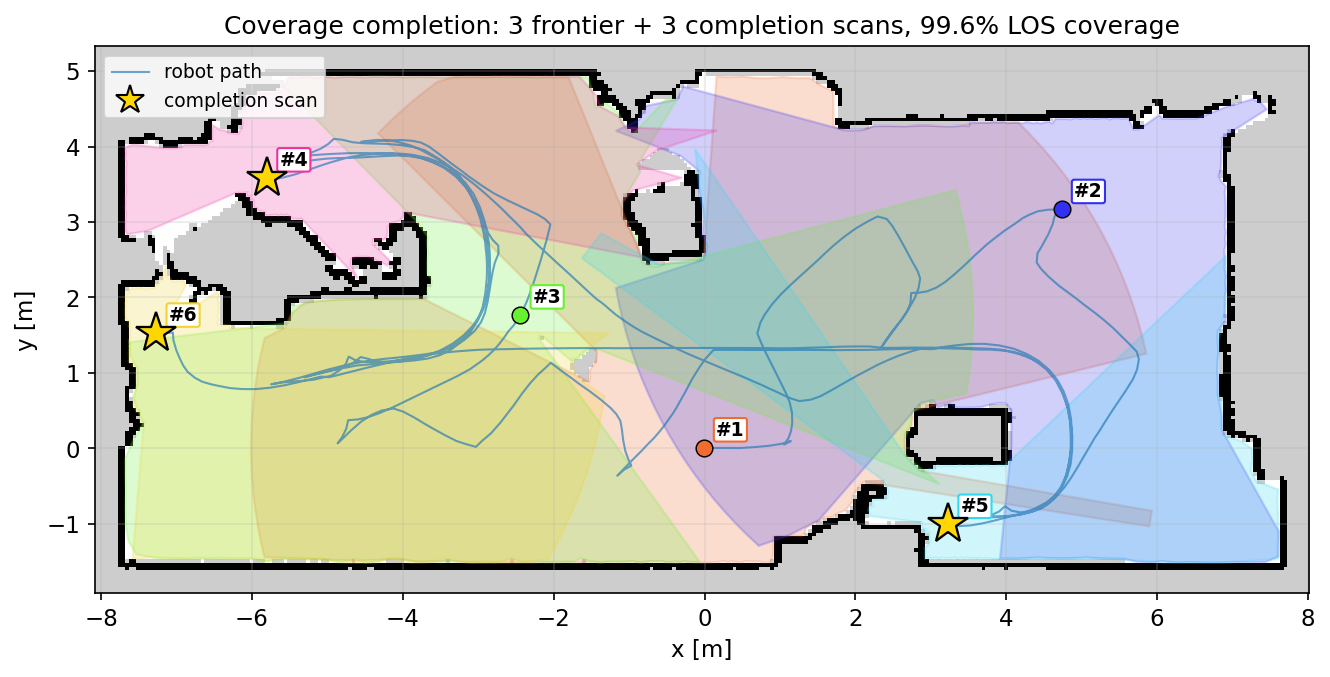
\includegraphics[width=0.7\linewidth]{figures/fig6_completion.png}
\caption{Coverage completion. After frontier exploration, the robot drives into
each still-uncovered pocket and scans ($\star$) until none above the minimum
pocket area remains. Here 3~frontier $+$ 3~completion scans, $99.6\%$ LOS.}
\label{fig:completion}
\end{figure}

\subsection{Parameter Sensitivity}

We characterize the two skip thresholds by deterministic replay of the
visibility policy over the same fixed paths as the ablation ($N=5$
single-room, $N=10$ multi-room paths); Figure~\ref{fig:sweep} reports means
with per-path standard deviations as error bars. Varying the relative
threshold $\tau$ over $[0.10,0.50]$ changes mean LOS coverage by at most about
two points (single-room $86.4\to84.3\%$; multi-room $85.2\to84.0\%$) and
mean scan count by less than one scan, so $\tau$ lies in a robust, flat
region and $\tau=0.30$ is not a sensitive choice. The absolute threshold
$A_{\min}$ is the operative knob that trades coverage against scan count. We
identify $A_{\min}=5$~m\textsuperscript{2} as the knee by the following
criterion: it is the largest threshold whose mean LOS remains within about
five points of the most aggressive setting
($A_{\min}=1$~m\textsuperscript{2}) in both environments (single-room $85.4$
versus $90.7\%$; multi-room $84.0$ versus $85.7\%$) while already halving
the scan count ($3.6$ versus $7.2$ scans in both environments). Beyond the
knee the trade turns unfavorable: pushing to
$A_{\min}=15$~m\textsuperscript{2} saves only about one further scan
($3.6\to2.2$ and $3.6\to2.8$) while coverage continues to erode
($85.4\to80.8\%$ and $84.0\to83.1\%$). This justifies the operating point
$\tau=0.30$, $A_{\min}=5$~m\textsuperscript{2}, which was fixed before the
hardware campaign.

\begin{figure}[H]
\centering
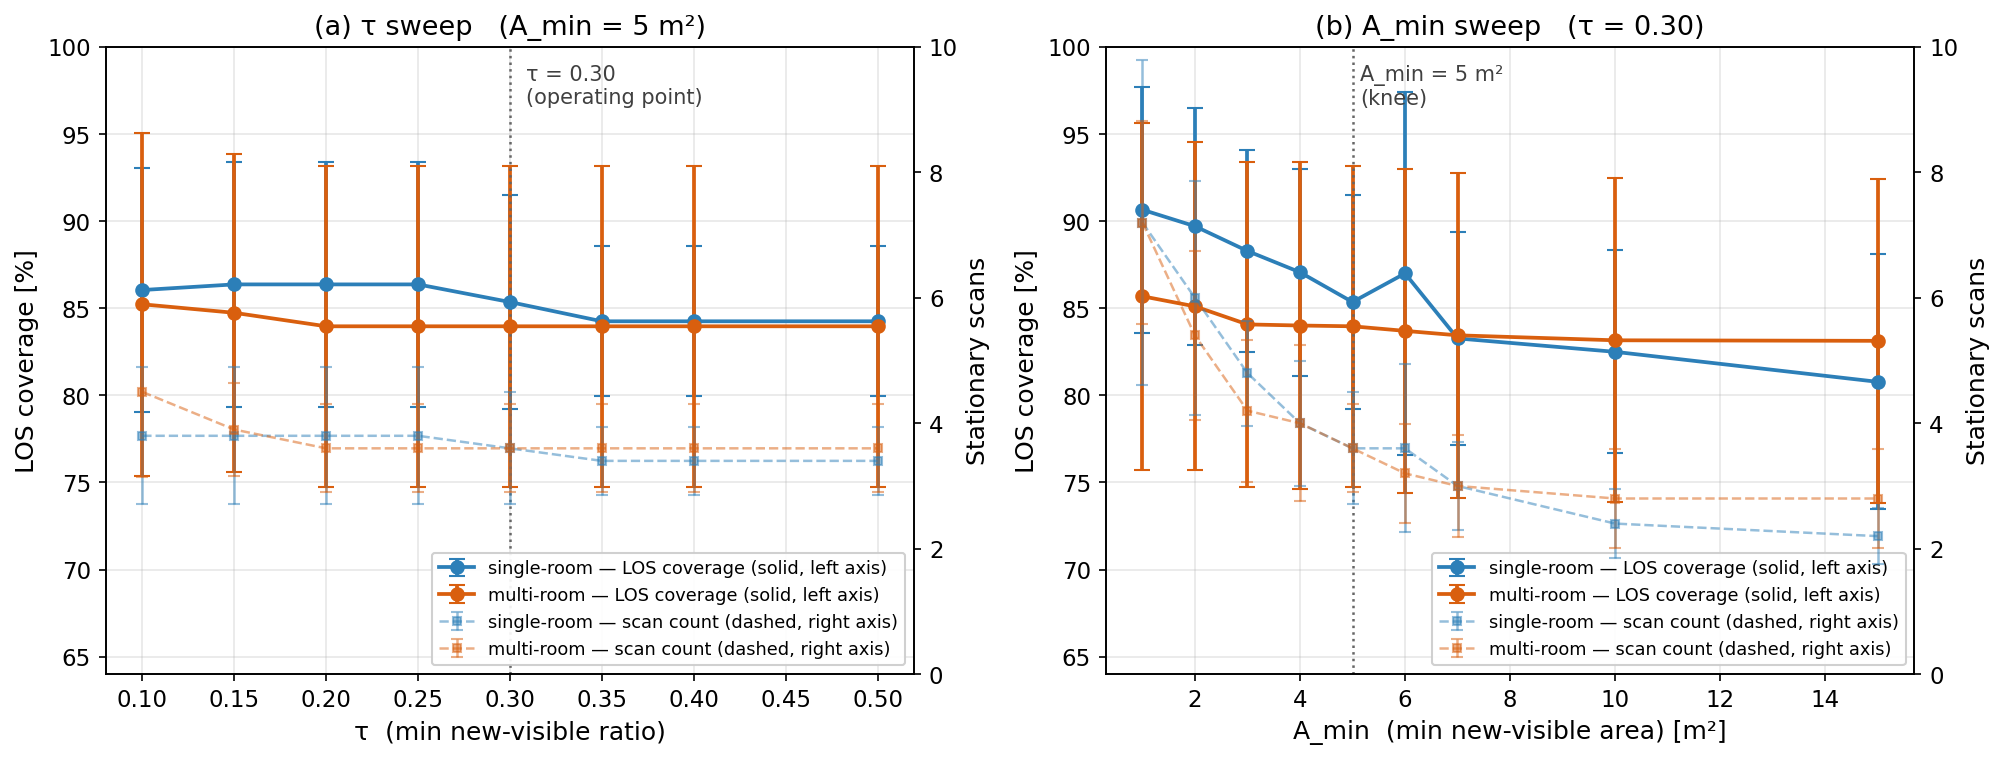
\includegraphics[width=0.95\linewidth]{figures/fig8_param_sweep.png}
\caption{Parameter sweep by deterministic replay on the fixed candidate
paths (mean~$\pm$~s.d.\ over $N=5$ single-room and $N=10$ multi-room paths).
Solid curves: LOS coverage (left axis); dashed curves: scan count (right
axis). (\textbf{a})~$\tau$ sweep at $A_{\min}=5$~m\textsuperscript{2};
(\textbf{b})~$A_{\min}$ sweep at $\tau=0.30$, knee marked.}
\label{fig:sweep}
\end{figure}

\subsection{Fully Autonomous On-Hardware Disk-Versus-Visibility Comparison}
\label{sec:fieldsim}

The preceding results characterize the placement policy in simulation. To test
whether this behavior carries over to the physical platform, we conducted a
fully autonomous on-hardware comparison in the industrial test room of
Figure~\ref{fig:testroom}: RedBOT04 explores the room live under frontier
exploration through the full Nav2 stack (MPPI controller) while Cartographer
builds the map online from the onboard 2D LiDAR, and the stop-and-scan sequencer
applies the placement policy of Section~\ref{sec:placement} in real time. At
each accepted pose the platform halts and the deck-mounted Leica BLK360~G1
acquires a full-dome stationary scan (Figure~\ref{fig:field}). Each
run is driven end to end by one skip rule---disk or visibility---so the
comparison exercises the entire pipeline, perception through placement through
scan acquisition, on real hardware. This is the same software stack used
throughout the simulation study, now running on the physical robot.

\begin{figure}[H]
\centering
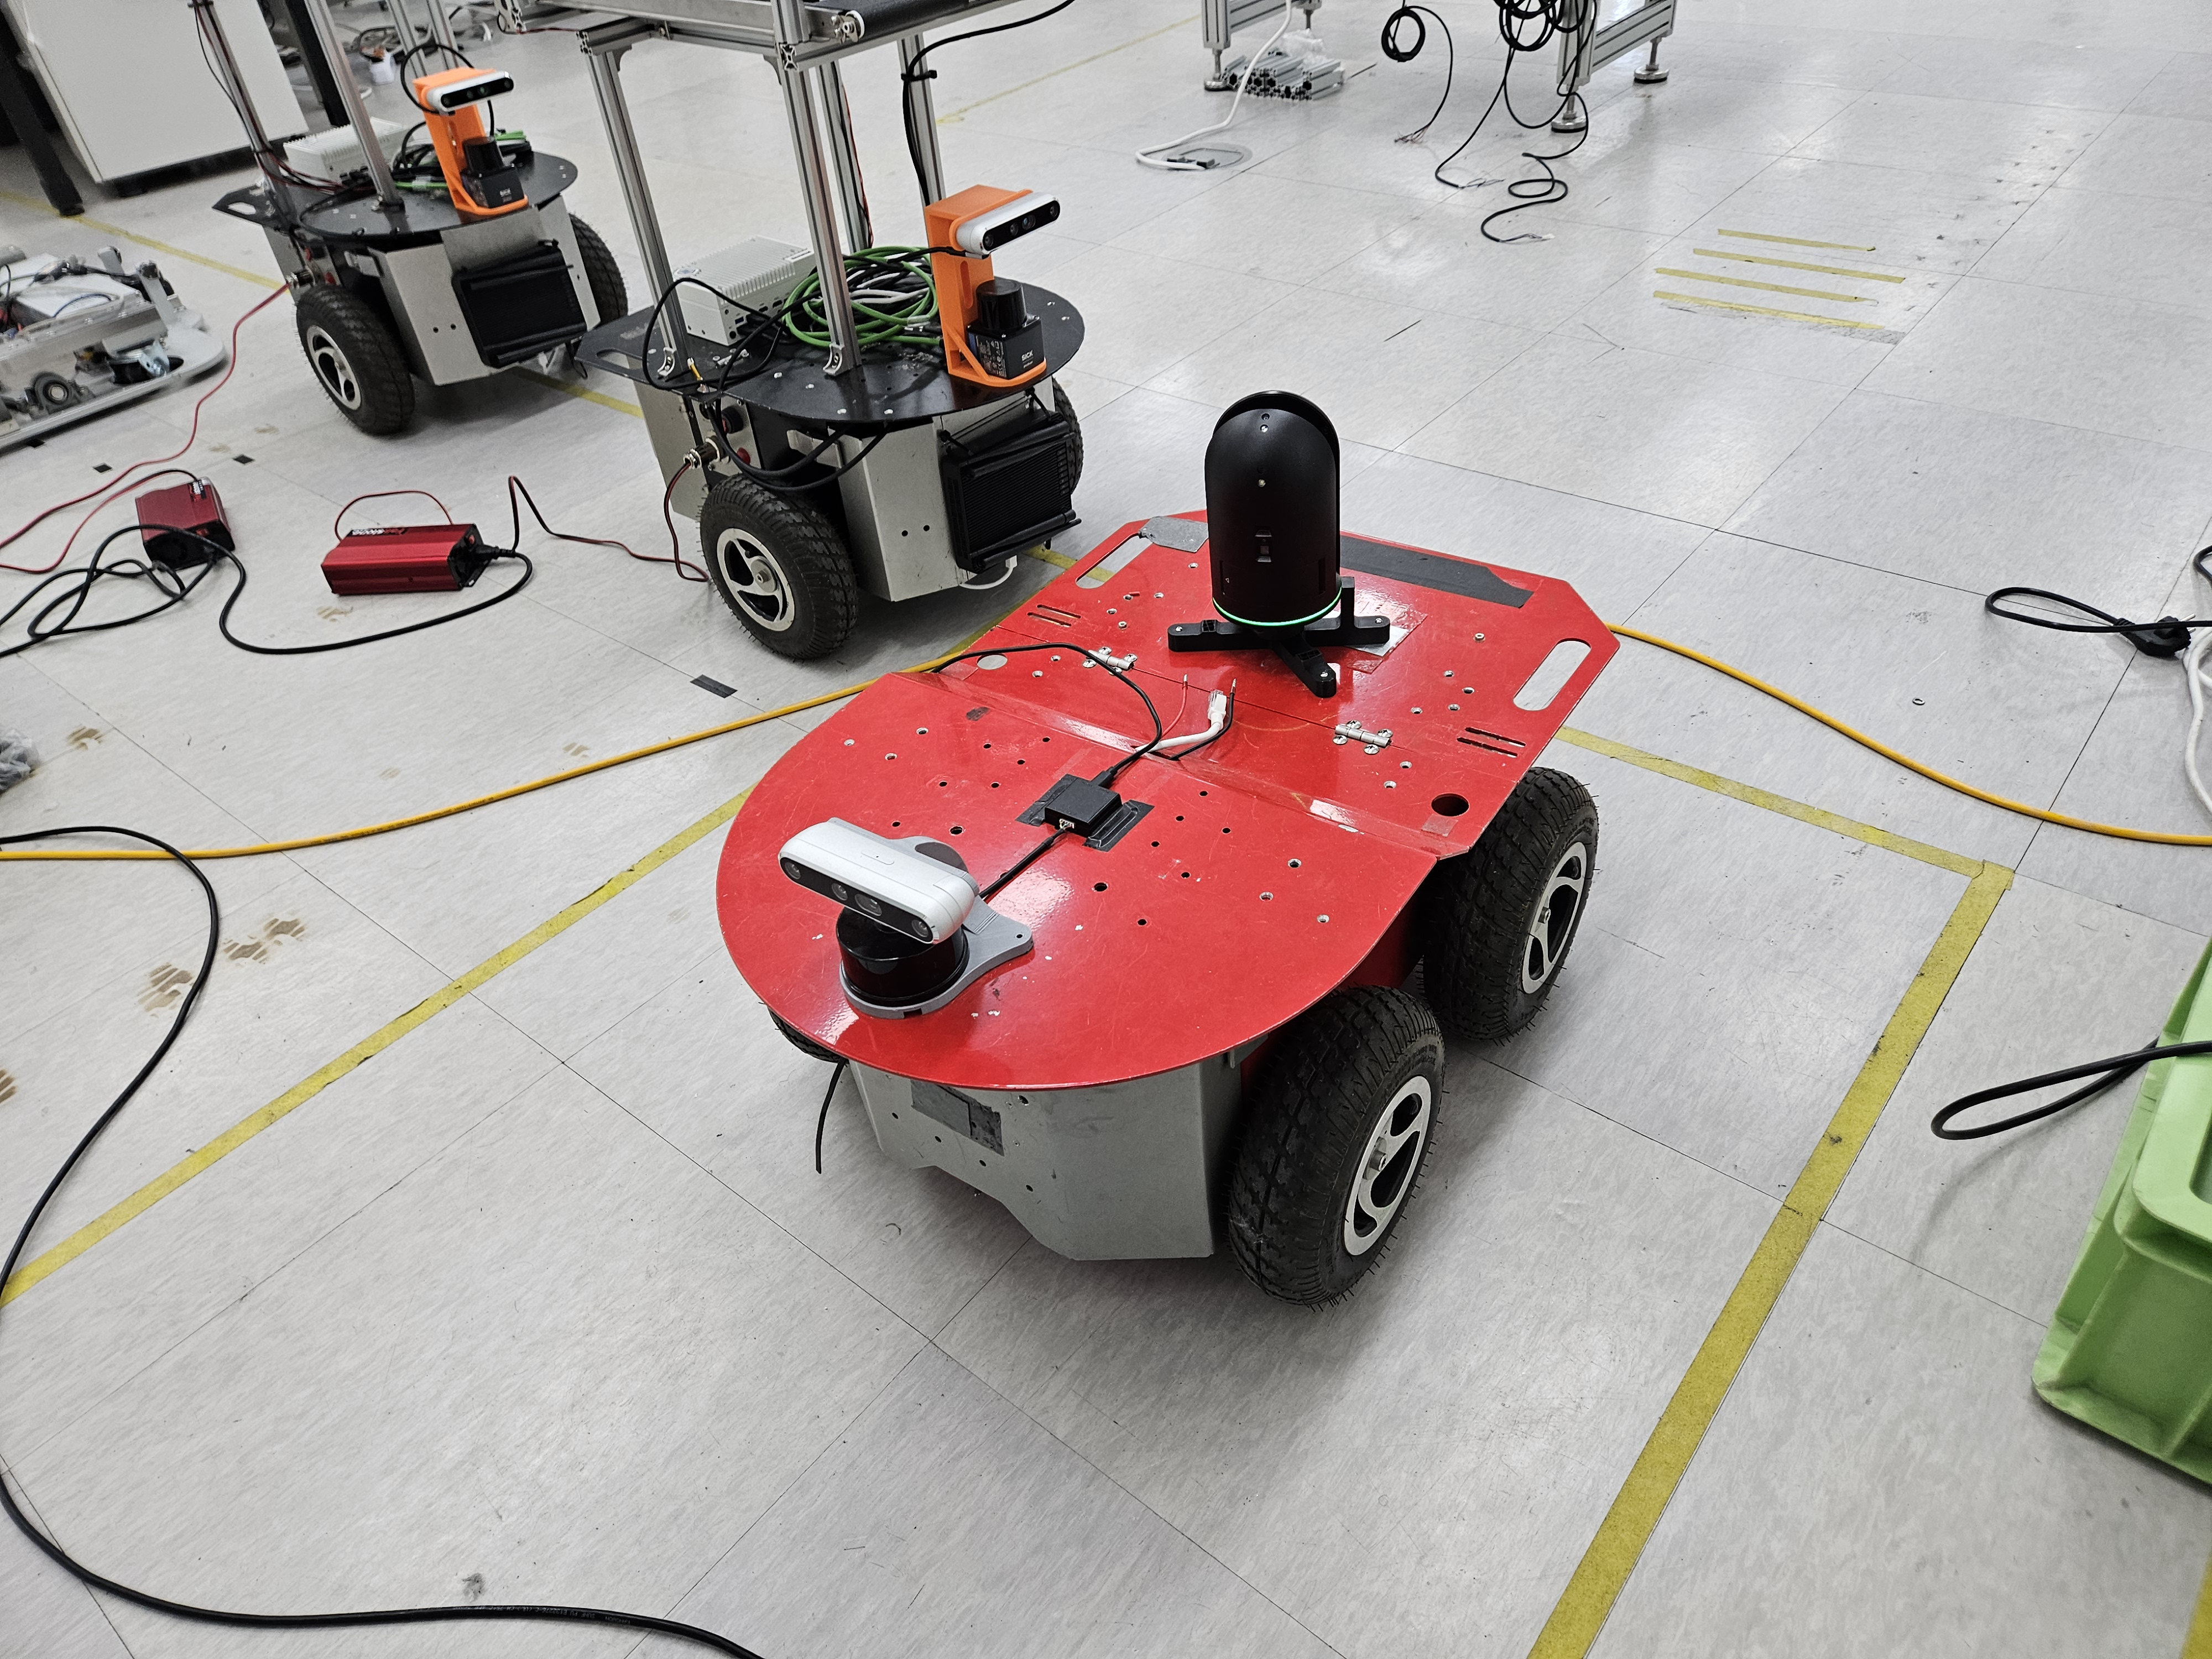
\includegraphics[width=0.82\linewidth]{figures/fig13_redbot04_field.jpg}
\caption{RedBOT04 deployed in the industrial test room during the fully
autonomous on-hardware runs, with the Leica BLK360 G1 mounted on its deck. The
platform navigates autonomously between scan stations and halts at each accepted
pose to acquire a stationary full-dome scan.}
\label{fig:field}
\end{figure}


Of the on-hardware exploration runs we retain the $N=4$ per policy (eight
completed runs in total) that completed a room-spanning traverse; two additional
early-terminated runs, in which frontier exploration stalled shortly after
start, are discarded as failed trials rather than policy samples. Because each live run maps a slightly different extent of free space,
we follow the common-reference protocol of Section~\ref{sec:setup}: every run is
evaluated on the single most complete SLAM map among the runs, so all runs share
one free-space denominator. Unlike the simulated ablation, hardware runs cannot
be paired---each is an independent live trial under one rule---so this
experiment complements the confound-free paired ablation with ecological
validity rather than replacing it. Table~\ref{tab:fieldsim} reports the
aggregate and Figure~\ref{fig:fieldsim} a representative run.

The outcome reproduces the controlled ablation on the physical platform---a
platform kinematically and dimensionally different from the simulated base,
indicating that the effect is a property of the coverage model rather than of
any particular robot. The
isotropic disk over-skips: it places only $1.8\pm0.5$ scans and, treating floor
behind the equipment island and furniture as covered, attains $77.6\pm10.5\%$ LOS
coverage with a large run-to-run variance, since whether its few stations happen
to see the occluded bays is largely incidental. The visibility rule recognizes the
occluded area as unseen, places $4.2\pm1.5$ scans, and covers $92.1\pm3.8\%$ of the
free space reliably---a far smaller run-to-run variance at the cost of about
two extra scans. Whether the scans these autonomous runs produce actually
register at survey grade is validated next (Section~\ref{sec:realhw}).

\begin{figure}[H]
\centering
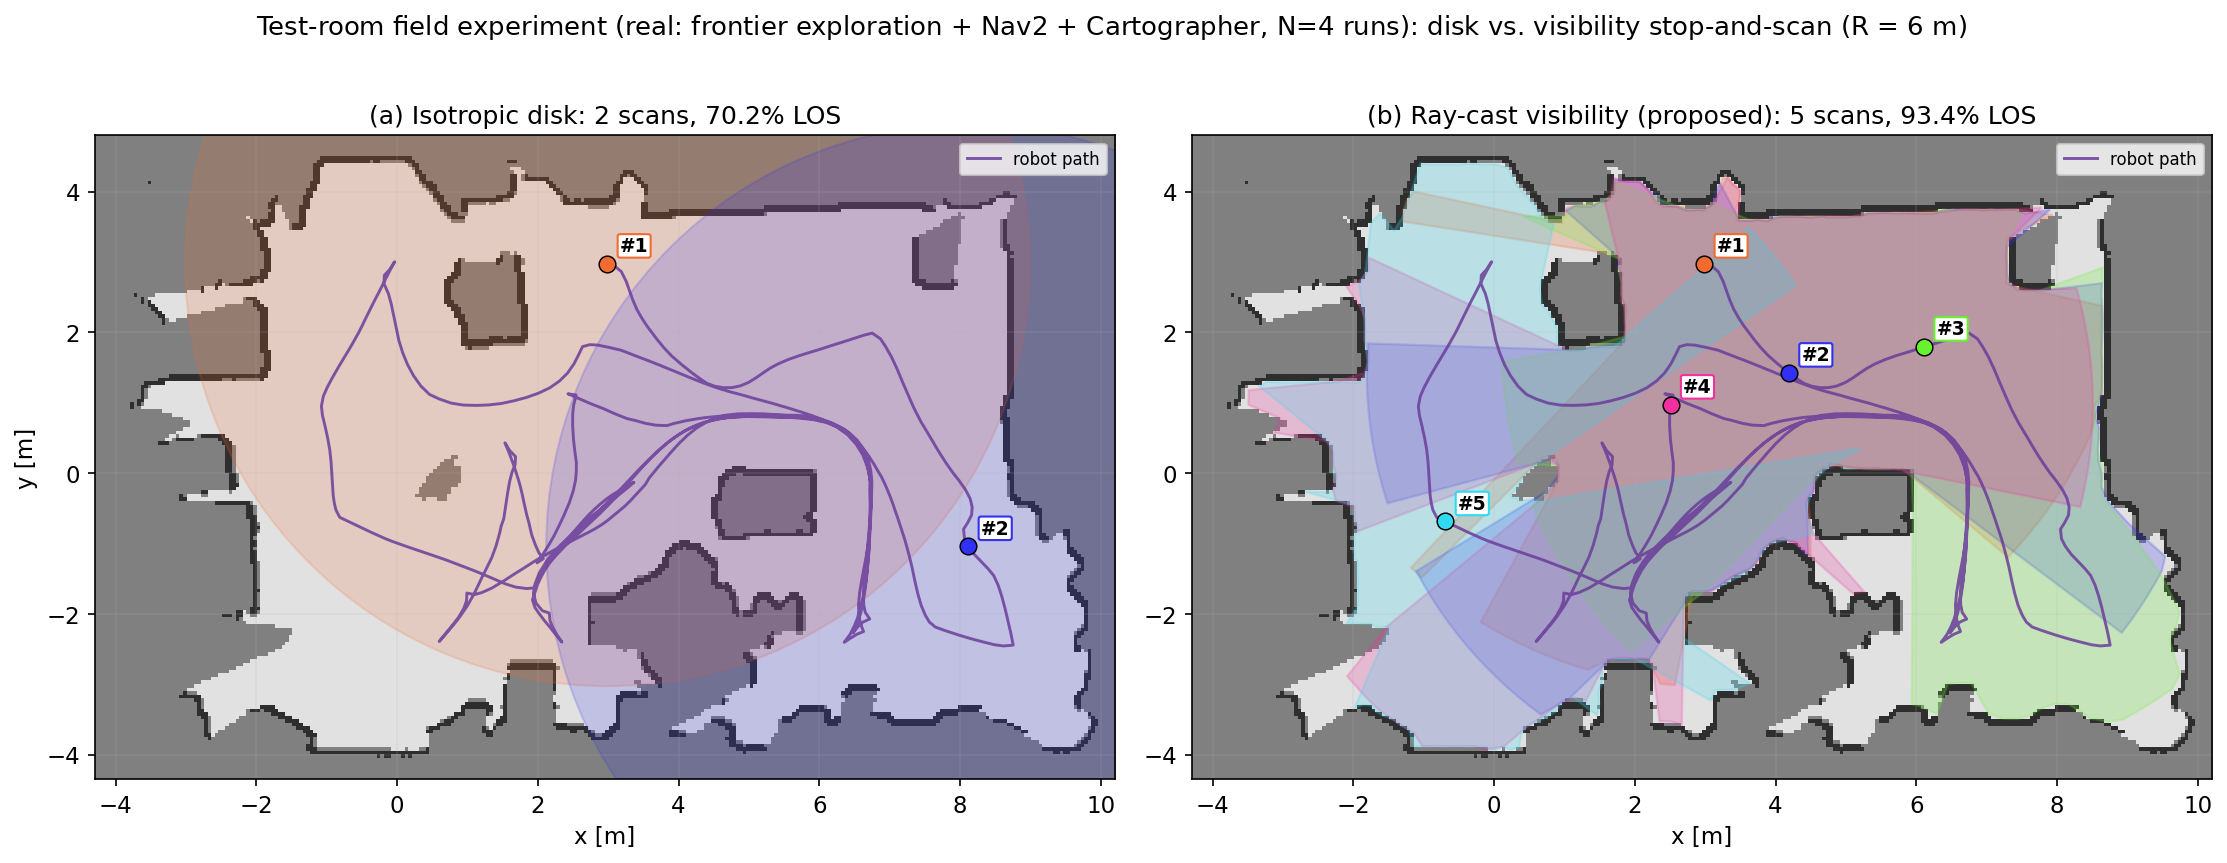
\includegraphics[width=\linewidth]{figures/fig14_testroom_fieldsim.png}
\caption{Fully autonomous on-hardware comparison in the physical test room
(representative runs; $R=6$~m). Light grey: mapped free space; dark grey:
unmapped; black: occupied; purple line: autonomous robot path; colored
markers: placed scans with their coverage regions. (\textbf{a})~Disk spacing
rule; (\textbf{b})~visibility rule.}
\label{fig:fieldsim}
\end{figure}

\begin{table}[H]
\caption{Fully autonomous on-hardware disk-versus-visibility comparison in the
physical test room ($N=4$ completed live frontier-exploration runs per policy on
RedBOT04, each driven end to end by one skip rule; all runs evaluated on the
common reference map). Values are mean~$\pm$~s.d.}
\label{tab:fieldsim}
\newcolumntype{Z}{>{\centering\arraybackslash}X}
\begin{tabularx}{\linewidth}{l Z Z}
\toprule
\textbf{Coverage model} & \textbf{Scans} & \textbf{LOS coverage (\%)} \\
\midrule
Isotropic disk (baseline)   & $1.8\pm0.5$ & $77.6\pm10.5$ \\
Ray-cast visibility (ours)  & $4.2\pm1.5$ & $\mathbf{92.1\pm3.8}$ \\
\bottomrule
\end{tabularx}
\noindent\footnotesize{BLK360 scans were acquired at every accepted pose in all
runs; the per-run offline registration of these scans is reported in
Section~\ref{sec:realhw}.}
\end{table}

\subsection{Survey-Grade Registration of the Autonomously Acquired Scans}
\label{sec:realhw}

The on-hardware comparison establishes where each rule scans; the remaining
question is whether the scans each rule produces meet the survey-grade
premise---that stationary scans placed to preserve line-of-sight overlap
register at survey grade on real data. To answer it, we registered the BLK360
scans of every completed run offline, each run as an independent project under
identical settings, in Leica Cyclone REGISTER~360 PLUS (BLK Edition) using
cloud-to-cloud alignment without artificial targets.
Registration is a post-mission batch step; importing and aligning one run's
network took on the order of minutes on a desktop workstation, small compared
with the acquisition time of the scans themselves.
Table~\ref{tab:registration} summarizes the per-run registration networks.

All four visibility runs registered at survey grade. Their networks comprise
$3$--$6$ setups joined by $3$--$13$ pairwise links, the bundle adjustments
converged at $4$--$5$~mm with overall overlaps of $84$--$88\%$, and every
individual link fell within the software's highest quality band (maximum error
$\le15$~mm; per-link overlaps $74$--$92\%$, errors $3$--$6$~mm). For a
scanner whose single-setup 3D point accuracy is on the order of a few
millimeters, a $4$--$5$~mm bundle error is at the level of the sensor noise
floor, i.e., registration adds essentially no error beyond the device itself.
The registered clouds reconstruct the room---display wall, equipment, and
floor---as a single coherent model: Figure~\ref{fig:regcloud} shows
interior views of the registered cloud of visibility run~3 along two diagonal
viewing directions, and Figure~\ref{fig:realreg} (top) the corresponding
scan-station network.

The disk runs tell a structurally different story. The three disk runs that
placed two scans each registered as a two-setup network with a single link
($75$--$85\%$ overlap, $2$~mm); the fourth disk run placed only one scan and
therefore admits no registration at all. The low single-link residuals should
not be read as superior registration: with one link there is no redundancy, so
the alignment is not cross-checked by any independent constraint, and the
resulting model covers correspondingly less of the room
(Section~\ref{sec:fieldsim}). The structural contrast is the point: the
visibility rule reliably produces redundant, bundle-verifiable multi-link
networks, whereas the disk rule yields at best a minimal single-link pair and
at worst a single unregistrable setup (Figure~\ref{fig:realreg}).

\begin{table}[H]
\caption{Per-run offline registration of the autonomously acquired scans
(Leica Cyclone REGISTER~360 PLUS, BLK Edition; cloud-to-cloud, no targets,
identical settings). Every link of every registered network lies within the
software's highest quality band (maximum error $\le15$~mm).}
\label{tab:registration}
\newcolumntype{Z}{>{\centering\arraybackslash}X}
\begin{tabularx}{\linewidth}{l l Z Z Z Z}
\toprule
\textbf{Policy} & \textbf{Run} & \textbf{Setups} & \textbf{Links} & \textbf{Overall overlap (\%)} & \textbf{Bundle error (mm)} \\
\midrule
Visibility & 1 & 3 & 3  & 86 & 5 \\
Visibility & 2 & 6 & 13 & 86 & 5 \\
Visibility & 3 & 5 & 10 & 84 & 5 \\
Visibility & 4 & 3 & 3  & 88 & 4 \\
\midrule
Disk & 1 & 1 & 0 & \multicolumn{2}{c}{not registrable (single setup)} \\
Disk & 2 & 2 & 1 & 75 & 2 \\
Disk & 3 & 2 & 1 & 85 & 2 \\
Disk & 4 & 2 & 1 & 84 & 2 \\
\bottomrule
\end{tabularx}
\end{table}

\begin{figure}[H]
\centering
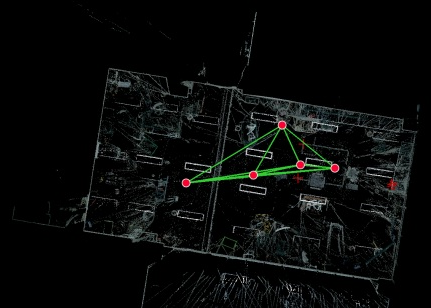
\includegraphics[height=5.0cm]{figures/fig15_reg_network_vis.png}\hfill
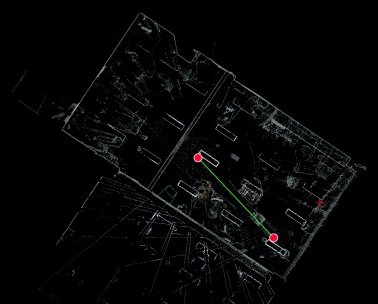
\includegraphics[height=5.0cm]{figures/fig16_reg_network_disk.png}
\caption{Registered scan-station networks (top-down view; red markers are
setup positions, green edges are cloud-to-cloud links of
Table~\ref{tab:registration}). (\textbf{Left})~Visibility run~3: five setups
joined by ten redundant links reconstruct the room as a single coherent model.
(\textbf{Right})~Disk run~4: two setups joined by a single link---a minimal
network with no redundant constraint, covering only part of the room.}
\label{fig:realreg}
\end{figure}

\begin{figure}[H]
\centering
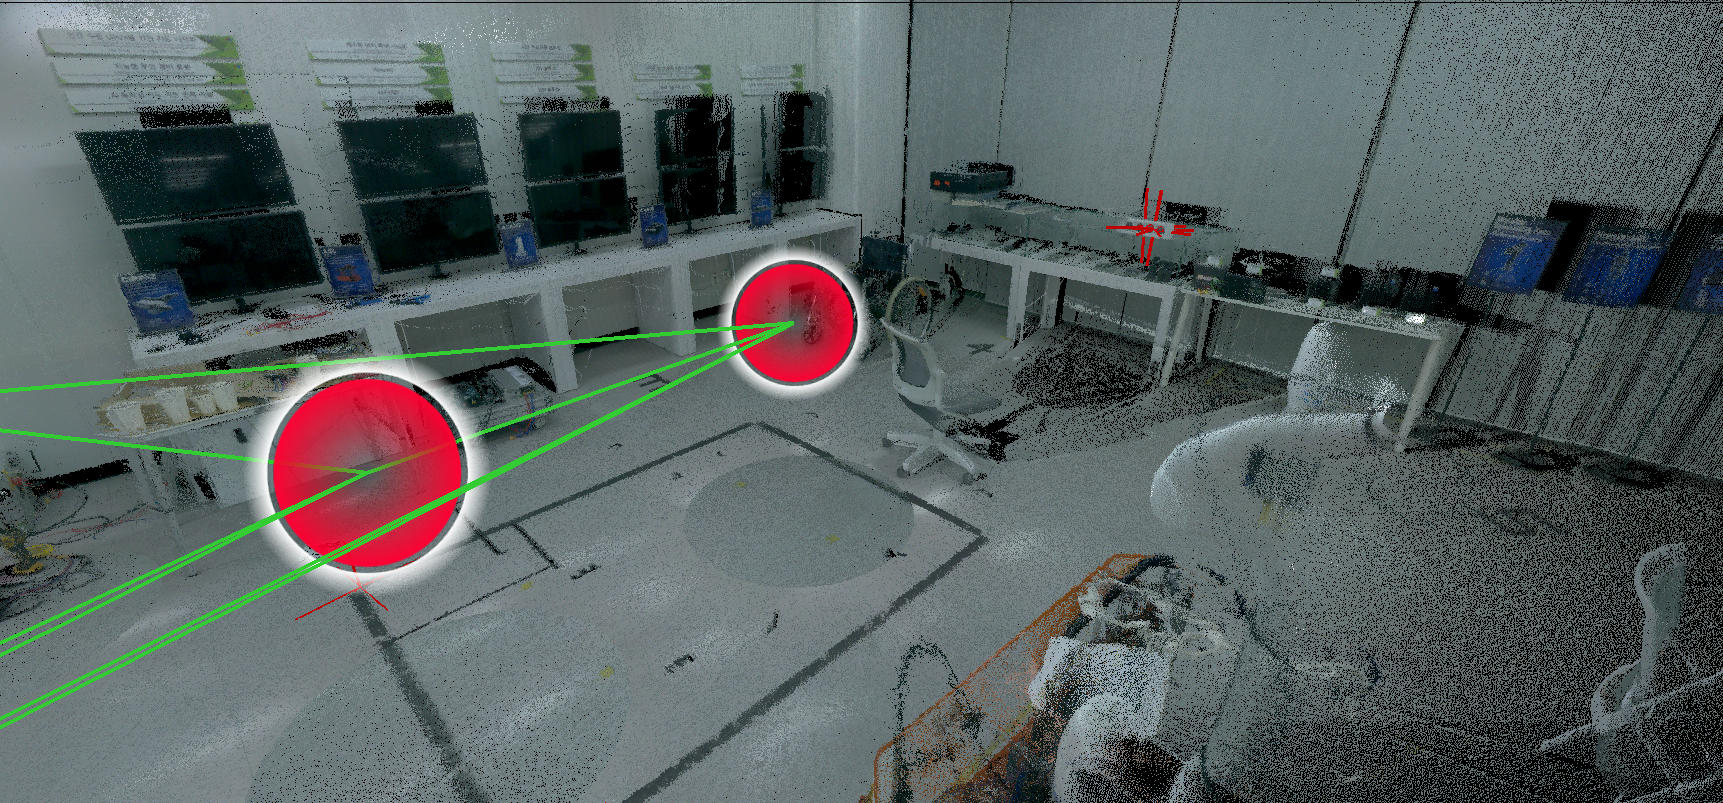
\includegraphics[width=0.49\linewidth]{figures/fig17_regcloud_wall.png}\hfill
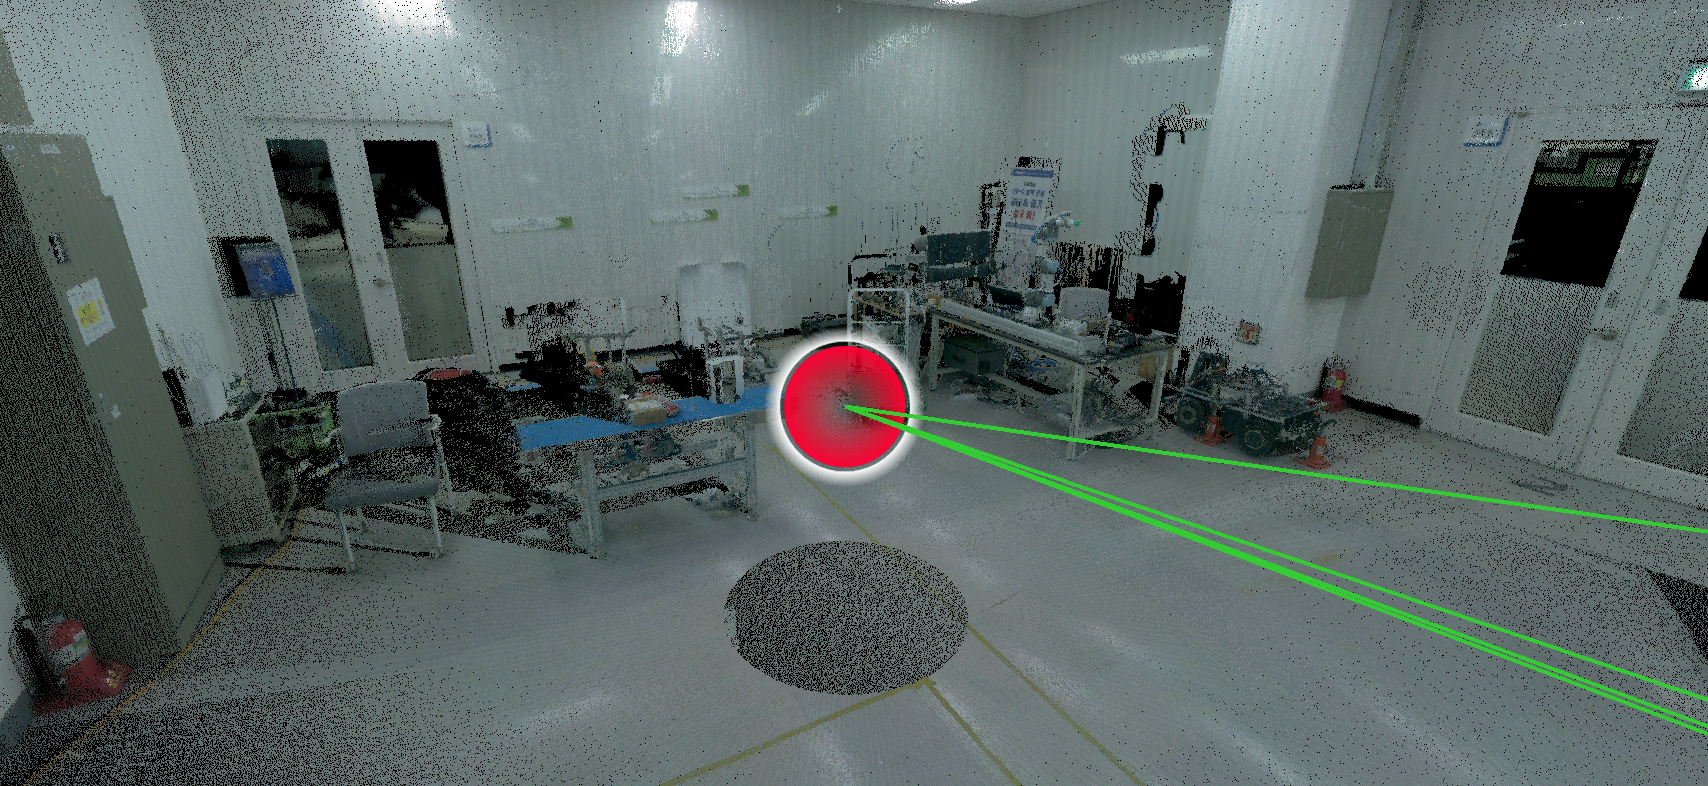
\includegraphics[width=0.49\linewidth]{figures/fig18_regcloud_equipment.png}
\caption{Interior views of the registered colorized point cloud of
visibility run~3 along two diagonal directions: toward the display wall
(\textbf{left}) and toward the equipment side (\textbf{right}). Red markers
and green edges are the scan stations and links of
Table~\ref{tab:registration}.}
\label{fig:regcloud}
\end{figure}

These results validate the workflow end to end on real hardware and confirm the
overlap rationale that motivates the visibility model: placement that keeps
successive stations in mutual line of sight consistently yields pairwise
overlaps well above the level at which cloud-to-cloud registration is reliable,
and the resulting bundles are survey grade in every visibility run. One remark
bounds the scope: bundle strengths are moderate ($38$--$48\%$) across runs,
reflecting the corridor-like traverses the explorer takes through the room; a
loop-closing or areal station layout would raise this redundancy measure, and
the placement policy's coverage-completion phase is a natural driver of such
layouts. Together with Section~\ref{sec:fieldsim}, this completes the chain of
evidence on the physical room: the live comparison establishes that the
visibility rule, not the disk rule, reliably produces high-LOS scan placements,
and the per-run registration establishes that those placements consistently
yield survey-grade, bundle-verifiable scan networks---while disk placements do
not even guarantee a registrable network. A downstream validation in which an
independent robot navigates the completed map to quantify localization accuracy
remains future work.

\section{Discussion}
\label{sec:discussion}

The controlled ablation isolates a single design choice, the coverage model used
for the scan/skip decision, and shows that occlusion-aware visibility yields
consistently higher LOS coverage than the Euclidean disk at the cost of one to
two additional scans per environment; the disk baseline run under the identical
marginal-gain rule performs even worse than the spacing rule in the multi-room
world, attributing the deficiency to the coverage model itself rather than to
the acceptance rule. The effect is structural rather than incidental:
the disk model is provably optimistic ($B\subseteq B_{\mathrm{disk}}$ always
holds, with equality only in obstacle-free surroundings), so wherever a wall lies within
range it over-claims coverage and suppresses a needed scan. The live multi-room
run makes the practical consequence vivid: counting a room through a partition
caps the disk policy at $46.9\%$ LOS, while the visibility policy scans each room.
The same pattern reappears on the physical platform: in the fully autonomous
on-hardware comparison in the industrial test room (Section~\ref{sec:fieldsim}),
the disk rule attains $77.6\pm10.5\%$ LOS with large run-to-run variance---whether
its few stations happen to see the occluded bays is incidental---whereas the
visibility rule reaches $92.1\pm3.8\%$ reliably, indicating that the effect is
not an artifact of simulation. Per-run registration of the acquired scans
(Section~\ref{sec:realhw}) extends the contrast to the survey product itself:
every visibility run yields a redundant, bundle-verifiable network at
$4$--$5$~mm, while the disk rule's sparse placements yield at best a single
uncorroborated link and at worst no registrable network at all.

Several limitations frame the result. First, the planning representation is
two-dimensional: visibility is evaluated on the occupancy grid at sensor
height, so vertical occlusions---shelves, overhangs, elevated machinery, or
surfaces stacked at different heights above the same floor cell---are not
modeled, and LOS coverage certifies floor-space sight lines rather than full
3D surface coverage (Section~\ref{sec:scope2d}). The robotic deployment adds
a related height effect: the deck-mounted scanner observes from roughly
$0.5$~m above the floor, lower than a typical tripod setup, so low furniture
and equipment cast longer horizontal shadows than in a manual survey of the
same room. This makes occlusion-aware placement more important on a robotic
platform, not less; but it also means the acquired clouds have a lower vantage
than a conventional tripod survey would provide. Extending the model to a
genuinely 3D visibility representation, for example on a voxel or octree map
or over reconstructed surfaces, is the principal direction for future work.
Second, even within its 2D scope, LOS coverage is a geometric proxy
for observation quality: it certifies an unobstructed sight line within the range
bound but does not model incidence angle, range-dependent point density, or
surface reflectivity, all of which affect the usefulness of a survey scan. A
visibility-weighted coverage that discounts grazing or far-range cells is a
natural refinement. Third, the controlled paired ablation is conducted in
simulation with a mock scanner, because hardware runs cannot be paired: each
live run sees its own map and trajectory. The real-hardware experiments narrow
this gap from two directions---the fully autonomous comparison of
Section~\ref{sec:fieldsim} reproduces the placement gain with each rule driving
the physical robot end to end, and Section~\ref{sec:realhw} registers every
run's scans independently, showing survey-grade networks in all visibility
runs---but the on-hardware comparison is by nature live and unpaired, so these
results complement rather than replace the confound-free ablation. A downstream
navigation validation, in which an independent robot localizes against the
completed map to quantify end-use accuracy, is left to future work.
Fourth, the visibility model presently assumes an optical line-of-sight sensor,
which is
appropriate for a TLS but not for the penetrating or dwell-time sensors that
share the stop-and-scan workflow.

This last point also indicates a path to generalization. The coverage model
treats the sensor as a fixed optical ray-caster, but the stop-and-scan family
spans sensors with very different observation models. A promising direction is to
attach a sensor-level semantic description, for example whether a sensor
penetrates obstacles and over what range and field of view, to the robot model,
and to let that description parameterize the ray-termination rule so that the same
placement policy adapts across heterogeneous stop-and-scan sensors without code
changes. Populating such descriptions automatically, e.g.\ from sensor
datasheets, and the downstream navigation validation on the completed map are
the focus of ongoing work.

\section{Conclusions}
\label{sec:conclusions}

We presented an occlusion-aware visibility coverage model for robotic
stop-and-scan 3D LiDAR mapping, together with a marginal-gain placement policy
built on it; the model performs 2D scan-station planning on the live occupancy
map for subsequent 3D mapping, and a survey-grade terrestrial laser scanner is
its experimental instantiation. Replacing the isotropic disk with a ray-cast
visibility region and scoring candidates by line-of-sight marginal gain
corrects the disk model's structural over-claiming of occluded space. In a physics-based simulation built
from a real scanner-derived environment, a controlled paired ablation that
isolates the skip decision showed that the visibility rule raises LOS coverage
from about $77\%$ to $84$--$85\%$ at the cost of one to two additional scans,
while a disk baseline governed by the identical marginal-gain rule performed no
better than the spacing rule in the single-room world and markedly worse in the
multi-room world ($59.1\%$ LOS), attributing the deficiency to the coverage
model itself; a live multi-room run improved coverage from $46.9\%$ to
$95.1\%$ relative to the disk model, and an optional coverage-completion phase
reached about $99\%$ LOS. A
parameter study showed the relative threshold is robust while the absolute-area
threshold is the operative coverage--scan trade-off knob. Beyond simulation, a fully
autonomous on-hardware comparison in an industrial test room, with each skip
rule driving the live exploration and scan acquisition of a four-wheeled
platform carrying a BLK360 G1, reproduced the placement gain
($77.6\to92.1\%$ LOS) on the physical robot; per-run offline registration showed
that every visibility run yields a survey-grade, redundant multi-link network
($4$--$5$~mm bundle error, $84$--$88\%$ overlap), whereas disk runs yield at
best a single-link network and at worst a single unregistrable scan. Future work will
refine LOS into a visibility-weighted coverage that accounts for incidence and
range, generalize the ray-termination rule to heterogeneous stop-and-scan sensors
via sensor-level semantic descriptions, extend the coverage model to a
genuinely 3D visibility representation (voxel-, octree-, or surface-based)
that captures vertical occlusion, and add a downstream navigation validation
in which an independent robot autonomously localizes against the completed
map. Within the room-scale indoor environments and the optical stop-and-scan
sensor class studied here, the evidence supports occlusion-aware visibility,
rather than Euclidean proximity, as the basis for deciding where a robot
should stop and scan.



%%%%%%%%%%%%%%%%%%%%%%%%%%%%%%%%%%%%%%%%%%
\section{Patents}

This section is not mandatory, but may be added if there are patents resulting from the work reported in this manuscript.

%%%%%%%%%%%%%%%%%%%%%%%%%%%%%%%%%%%%%%%%%%
\vspace{6pt} 

%%%%%%%%%%%%%%%%%%%%%%%%%%%%%%%%%%%%%%%%%%
%% optional
%\supplementary{The following supporting information can be downloaded at:  \linksupplementary{s1}, Figure S1: title; Table S1: title; Video S1: title.}

% Only for journal Methods and Protocols:
% If you wish to submit a video article, please do so with any other supplementary material.
% \supplementary{The following supporting information can be downloaded at: \linksupplementary{s1}, Figure S1: title; Table S1: title; Video S1: title. A supporting video article is available at doi: link.}

% Only used for preprtints:
% \supplementary{The following supporting information can be downloaded at the website of this paper posted on \href{https://www.preprints.org/}{Preprints.org}.}

% Only for journal Hardware:
% If you wish to submit a video article, please do so with any other supplementary material.
% \supplementary{The following supporting information can be downloaded at: \linksupplementary{s1}, Figure S1: title; Table S1: title; Video S1: title.\vspace{6pt}\\
%\begin{tabularx}{\textwidth}{lll}
%\toprule
%\textbf{Name} & \textbf{Type} & \textbf{Description} \\
%\midrule
%S1 & Python script (.py) & Script of python source code used in XX \\
%S2 & Text (.txt) & Script of modelling code used to make Figure X \\
%S3 & Text (.txt) & Raw data from experiment X \\
%S4 & Video (.mp4) & Video demonstrating the hardware in use \\
%... & ... & ... \\
%\bottomrule
%\end{tabularx}
%}

%%%%%%%%%%%%%%%%%%%%%%%%%%%%%%%%%%%%%%%%%%
\authorcontributions{Conceptualization, S.K. and T.-Y.K.; methodology, S.K.; software, S.K.; validation, S.K.; formal analysis, S.K.; investigation, S.K. and Y.S.; resources, B.K.; data curation, Y.S.; writing---original draft preparation, S.K.; writing---review and editing, S.K. and T.-Y.K.; visualization, S.K.; supervision, T.-Y.K.; project administration, T.-Y.K. All authors have read and agreed to the published version of the manuscript.}

\funding{This research received no external funding.}

\institutionalreview{Not applicable.}

\informedconsent{Not applicable.

Written informed consent for publication must be obtained from participating patients who can be identified (including by the patients themselves). Please state ``Written informed consent has been obtained from the patient(s) to publish this paper'' if applicable.}

\dataavailability{The source code and simulation assets supporting this study are available from the corresponding author upon reasonable request and will be released publicly upon publication.} 

%\durcstatement{Current research is limited to the [please insert a specific academic field, e.g., XXX], which is beneficial [share benefits and/or primary use] and does not pose a threat to public health or national security. Authors acknowledge the dual-use potential of the research involving xxx and confirm that all necessary precautions have been taken to prevent potential misuse. As an ethical responsibility, authors strictly adhere to relevant national and international laws about DURC. Authors advocate for responsible deployment, ethical considerations, regulatory compliance, and transparent reporting to mitigate misuse risks and foster beneficial outcomes.}

% Only for journal Nursing Reports
%\publicinvolvement{Please describe how the public (patients, consumers, carers) were involved in the research. Consider reporting against the GRIPP2 (Guidance for Reporting Involvement of Patients and the Public) checklist. If the public were not involved in any aspect of the research add: ``No public involvement in any aspect of this research''.}
%
%% Only for journal Nursing Reports
%\guidelinesstandards{Please add a statement indicating which reporting guideline was used when drafting the report. For example, ``This manuscript was drafted against the XXX (the full name of reporting guidelines and citation) for XXX (type of research) research''. A complete list of reporting guidelines can be accessed via the equator network: \url{https://www.equator-network.org/}.}
%
%% Only for journal Nursing Reports
%\useofartificialintelligence{Please describe in detail any and all uses of artificial intelligence (AI) or AI-assisted tools used in the preparation of the manuscript. This may include, but is not limited to, language translation, language editing and grammar, or generating text. Alternatively, please state that “AI or AI-assisted tools were not used in drafting any aspect of this manuscript”.}

\acknowledgments{The authors thank the members of the Control and Robotics Laboratory at Sungkyunkwan University for helpful discussions. During the preparation of this manuscript, the authors used a generative AI assistant (Claude, Anthropic) for language editing and LaTeX formatting; the authors have reviewed and edited all output and take full responsibility for the content of this publication.}

\conflictsofinterest{Authors Sangmin Kim and Byeongjun Kim are employed by CASELAB Co., Ltd.; author Yonghyeon Song contributed to this work as an intern at CASELAB Co., Ltd.; and author Tae-Yong Kuc is the chief executive officer of CASELAB Co., Ltd. The authors declare no other conflicts of interest.} 

%%%%%%%%%%%%%%%%%%%%%%%%%%%%%%%%%%%%%%%%%%
%% Optional

%% Only for journal Encyclopedia
%\entrylink{The Link to this entry published on the encyclopedia platform.}

\abbreviations{Abbreviations}{
The following abbreviations are used in this manuscript:
\\

\noindent 
\begin{tabular}{@{}ll}
TLS & Terrestrial laser scanner\\
LiDAR & Light detection and ranging\\
LOS & Line of sight\\
NBV & Next-best-view\\
SLAM & Simultaneous localization and mapping\\
MPPI & Model predictive path integral\\
GPR & Ground-penetrating radar\\
BIM & Building information model
\end{tabular}
}

%%%%%%%%%%%%%%%%%%%%%%%%%%%%%%%%%%%%%%%%%%
%% Optional appendix removed (no appendix in this manuscript)

%%%%%%%%%%%%%%%%%%%%%%%%%%%%%%%%%%%%%%%%%%
%\isPreprints{}{% This command is only used for ``preprints''.
\begin{adjustwidth}{-\extralength}{0cm}
%} % If the paper is ``preprints'', please uncomment this parenthesis.
%\printendnotes[custom] % Un-comment to print a list of endnotes

\reftitle{References}

% Please provide the correct journal abbreviation (e.g. according to the “List of Title Word Abbreviations” http://www.issn.org/services/online-services/access-to-the-ltwa/).
% Citations and References in Supplementary files are permitted provided that they also appear in the reference list here. 

%=====================================
% References, variant A: external bibliography
%=====================================
% \bibliography{your_external_BibTeX_file}

%=====================================
% References, variant B: internal bibliography
%=====================================

% ACS format
\begin{thebibliography}{99}

\bibitem{leica-blk360}
Leica Geosystems. \textit{Leica BLK360 Imaging Laser Scanner: Product Specifications}; Leica Geosystems AG: Heerbrugg, Switzerland, 2022. Available online: \url{https://shop.leica-geosystems.com/leica-blk/blk360} (accessed on 15 June 2026).

\bibitem{stopandgo-review}
Lin, Y.; Hyypp\"a, J.; Kukko, A. Stop-and-Go Mode: Sensor Manipulation as Essential as Sensor Development in Terrestrial Laser Scanning. \textit{Sensors} \textbf{2013}, \textit{13}, 8140--8154.

\bibitem{stopandgo-registration}
Park, S.; Ju, S.; Nguyen, M.H.; Yoon, S.; Heo, J. Automated Point Cloud Registration Approach Optimized for a Stop-and-Go Scanning System. \textit{Sensors} \textbf{2024}, \textit{24}, 138.

\bibitem{tls-scanplanning}
Aryan, A.; Bosch\'e, F.; Tang, P. Planning for terrestrial laser scanning in construction: A review. \textit{Autom. Constr.} \textbf{2021}, \textit{125}, 103551.

\bibitem{prieto2017nbs}
Prieto, S.A.; Quintana, B.; Adán, A.; Vázquez, A.S. As-is building-structure reconstruction from a probabilistic next best scan approach. \textit{Robot. Auton. Syst.} \textbf{2017}, \textit{94}, 186--207.

\bibitem{mozaffar2016occlusion}
Heidari Mozaffar, M.; Varshosaz, M. Optimal placement of a terrestrial laser scanner with an emphasis on reducing occlusions. \textit{Photogramm. Rec.} \textbf{2016}, \textit{31}, 374--393.

\bibitem{gas-coverage}
Arain, M.A.; Trincavelli, M.; Cirillo, M.; Schaffernicht, E.; Lilienthal, A.J. Global Coverage Measurement Planning Strategies for Mobile Robots Equipped with a Remote Gas Sensor. \textit{Sensors} \textbf{2015}, \textit{15}, 6845--6871.

\bibitem{robotic-ndt}
Halder, S.; Afsari, K. Robots in Inspection and Monitoring of Buildings and Infrastructure: A Systematic Review. \textit{Appl. Sci.} \textbf{2023}, \textit{13}, 2304.

\bibitem{iccas2026}
Kim, S.; Choi, J.-H.; An, Y.-C.; Kuc, T.-Y. Coverage-Aware Stop-and-Scan Frontier Exploration for Automated Survey-Grade 3D Mapping. Submitted to the \textit{2026 International Conference on Control, Automation and Systems (ICCAS)}, Sapporo, Japan, 27--30 October 2026; under review.

\bibitem{placed2023}
Placed, J.A.; Strader, J.; Carrillo, H.; Atanasov, N.; Indelman, V.; Carlone, L.; Castellanos, J.A. A Survey on Active Simultaneous Localization and Mapping: State of the Art and New Frontiers. \textit{IEEE Trans. Robot.} \textbf{2023}, \textit{39}, 1686--1705.

\bibitem{lluvia2021}
Lluvia, I.; Lazkano, E.; Ansuategi, A. Active Mapping and Robot Exploration: A Survey. \textit{Sensors} \textbf{2021}, \textit{21}, 2445.

\bibitem{yamauchi1997}
Yamauchi, B. A frontier-based approach for autonomous exploration. In \textit{Proceedings of the IEEE International Symposium on Computational Intelligence in Robotics and Automation (CIRA)}, Monterey, CA, USA, 10--11 July 1997; pp. 146--151.

\bibitem{umari2017}
Umari, H.; Mukhopadhyay, S. Autonomous robotic exploration based on multiple rapidly-exploring randomized trees. In \textit{Proceedings of the IEEE/RSJ International Conference on Intelligent Robots and Systems (IROS)}, Vancouver, BC, Canada, 24--28 September 2017; pp. 1396--1402.

\bibitem{connolly1985}
Connolly, C. The determination of next best views. In \textit{Proceedings of the IEEE International Conference on Robotics and Automation (ICRA)}, St.\ Louis, MO, USA, 25--28 March 1985; Volume 2, pp. 432--435.

\bibitem{bircher2016}
Bircher, A.; Kamel, M.; Alexis, K.; Oleynikova, H.; Siegwart, R. Receding horizon ``next-best-view'' planner for 3D exploration. In \textit{Proceedings of the IEEE International Conference on Robotics and Automation (ICRA)}, Stockholm, Sweden, 16--21 May 2016; pp. 1462--1468.

\bibitem{he2025}
He, Z.; et al. Enhancing autonomous exploration for robotics via real-time map optimization and improved frontier costs. \textit{Sci. Rep.} \textbf{2025}, \textit{15}.

\bibitem{quin2021}
Quin, P.; Nguyen, D.D.K.; Vu, T.L.; Alempijevic, A.; Paul, G. Approaches for Efficiently Detecting Frontier Cells in Robotics Exploration. \textit{Front. Robot. AI} \textbf{2021}, \textit{8}, 616470.

\bibitem{schmid2020}
Schmid, L.; Pantic, M.; Khanna, R.; Ott, L.; Siegwart, R.; Nieto, J. An Efficient Sampling-Based Method for Online Informative Path Planning in Unknown Environments. \textit{IEEE Robot. Autom. Lett.} \textbf{2020}, \textit{5}, 1500--1507.

\bibitem{zhou2021}
Zhou, B.; Zhang, Y.; Chen, X.; Shen, S. FUEL: Fast UAV Exploration Using Incremental Frontier Structure and Hierarchical Planning. \textit{IEEE Robot. Autom. Lett.} \textbf{2021}, \textit{6}, 779--786.

\bibitem{gonzalez2002}
Gonz\'alez-Ba\~nos, H.H.; Latombe, J.-C. Navigation Strategies for Exploring Indoor Environments. \textit{Int. J. Robot. Res.} \textbf{2002}, \textit{21}, 829--848.

\bibitem{galceran2013}
Galceran, E.; Carreras, M. A survey on coverage path planning for robotics. \textit{Robot. Auton. Syst.} \textbf{2013}, \textit{61}, 1258--1276.

\bibitem{choset2001}
Choset, H. Coverage for robotics---A survey of recent results. \textit{Ann. Math. Artif. Intell.} \textbf{2001}, \textit{31}, 113--126.

\bibitem{almadhoun2019}
Almadhoun, R.; Taha, T.; Seneviratne, L.; Zweiri, Y. A survey on multi-robot coverage path planning for model reconstruction and mapping. \textit{SN Appl. Sci.} \textbf{2019}, \textit{1}, 847.

\bibitem{hess2016}
Hess, W.; Kohler, D.; Rapp, H.; Andor, D. Real-time loop closure in 2D LIDAR SLAM. In \textit{Proceedings of the IEEE International Conference on Robotics and Automation (ICRA)}, Stockholm, Sweden, 16--21 May 2016; pp. 1271--1278.

\bibitem{macenski2020}
Macenski, S.; Mart\'in, F.; White, R.; Gin\'es Clavero, J. The Marathon 2: A Navigation System. In \textit{Proceedings of the IEEE/RSJ International Conference on Intelligent Robots and Systems (IROS)}, Las Vegas, NV, USA, 24 October 2020--24 January 2021; pp. 2718--2725.

\bibitem{guler2024}
G\"uler, M. frontier\_exploration\_ros2: A Modern C++ Frontier Exploration Package for ROS 2. Open-source software, 2026. Available online: \url{https://github.com/mertgulerx/frontier_exploration_ros2} (accessed on 15 June 2026).

\bibitem{orourke1987}
O'Rourke, J. \textit{Art Gallery Theorems and Algorithms}; Oxford University Press: New York, NY, USA, 1987.

\bibitem{urrutia2000}
Urrutia, J. Art gallery and illumination problems. In \textit{Handbook of Computational Geometry}; Sack, J.-R., Urrutia, J., Eds.; North-Holland: Amsterdam, The Netherlands, 2000; pp. 973--1027.

\bibitem{scott2003}
Scott, W.R.; Roth, G.; Rivest, J.-F. View planning for automated three-dimensional object reconstruction and inspection. \textit{ACM Comput. Surv.} \textbf{2003}, \textit{35}, 64--96.

\bibitem{tarabanis1995}
Tarabanis, K.A.; Allen, P.K.; Tsai, R.Y. A survey of sensor planning in computer vision. \textit{IEEE Trans. Robot. Autom.} \textbf{1995}, \textit{11}, 86--104.

\bibitem{zeng2020}
Zeng, R.; Wen, Y.; Zhao, W.; Liu, Y.-J. View Planning in Robot Active Vision: A Survey of Systems, Algorithms, and Applications. \textit{Comput. Vis. Media} \textbf{2020}, \textit{6}, 225--245.

\bibitem{dehbi2021}
Dehbi, Y.; Leonhardt, J.; Oehrlein, J.; Haunert, J.-H. Optimal Scan Planning with Enforced Network Connectivity for the Acquisition of Three-Dimensional Indoor Models. \textit{ISPRS J. Photogramm. Remote Sens.} \textbf{2021}, \textit{180}, 103--116.

\bibitem{knechtel2025}
Knechtel, J.; Dehbi, Y.; Klingbeil, L.; Haunert, J.-H. Simultaneous Planning of Standpoints and Routing for Laser Scanning of Buildings with Network Redundancy. \textit{ISPRS J. Photogramm. Remote Sens.} \textbf{2025}, \textit{224}, 59--74.

\bibitem{stachniss2005}
Stachniss, C.; Grisetti, G.; Burgard, W. Information gain-based exploration using Rao-Blackwellized particle filters. In \textit{Proceedings of Robotics: Science and Systems (RSS)}, Cambridge, MA, USA, 8--11 June 2005; pp. 65--72.

\bibitem{burgard2005}
Burgard, W.; Moors, M.; Stachniss, C.; Schneider, F.E. Coordinated multi-robot exploration. \textit{IEEE Trans. Robot.} \textbf{2005}, \textit{21}, 376--386.

\bibitem{elfes1989}
Elfes, A. Using occupancy grids for mobile robot perception and navigation. \textit{Computer} \textbf{1989}, \textit{22}, 46--57.

\bibitem{thrun2005}
Thrun, S.; Burgard, W.; Fox, D. \textit{Probabilistic Robotics}; MIT Press: Cambridge, MA, USA, 2005.

\bibitem{koenig2004}
Koenig, N.; Howard, A. Design and use paradigms for Gazebo, an open-source multi-robot simulator. In \textit{Proceedings of the IEEE/RSJ International Conference on Intelligent Robots and Systems (IROS)}, Sendai, Japan, 28 September--2 October 2004; pp. 2149--2154.

\bibitem{williams2016}
Williams, G.; Drews, P.; Goldfain, B.; Rehg, J.M.; Theodorou, E.A. Aggressive driving with model predictive path integral control. In \textit{Proceedings of the IEEE International Conference on Robotics and Automation (ICRA)}, Stockholm, Sweden, 16--21 May 2016; pp. 1433--1440.

\end{thebibliography}

% If authors have biography, please use the format below
%\section*{Short Biography of Authors}
%\bio
%{\raisebox{-0.35cm}{\includegraphics[width=3.5cm,height=5.3cm,clip,keepaspectratio]{Definitions/author1.pdf}}}
%{\textbf{Firstname Lastname} Biography of first author}
%
%\bio
%{\raisebox{-0.35cm}{\includegraphics[width=3.5cm,height=5.3cm,clip,keepaspectratio]{Definitions/author2.jpg}}}
%{\textbf{Firstname Lastname} Biography of second author}

% For the MDPI journals use author-date citation, please follow the formatting guidelines on http://www.mdpi.com/authors/references
% To cite two works by the same author: \citeauthor{ref-journal-1a} (\citeyear{ref-journal-1a}, \citeyear{ref-journal-1b}). This produces: Whittaker (1967, 1975)
% To cite two works by the same author with specific pages: \citeauthor{ref-journal-3a} (\citeyear{ref-journal-3a}, p. 328; \citeyear{ref-journal-3b}, p.475). This produces: Wong (1999, p. 328; 2000, p. 475)

%%%%%%%%%%%%%%%%%%%%%%%%%%%%%%%%%%%%%%%%%%
%% for journal Sci
%\reviewreports{\\
%Reviewer 1 comments and authors’ response\\
%Reviewer 2 comments and authors’ response\\
%Reviewer 3 comments and authors’ response
%}
%%%%%%%%%%%%%%%%%%%%%%%%%%%%%%%%%%%%%%%%%%
\PublishersNote{}
%\isPreprints{}{% This command is only used for ``preprints''.
\end{adjustwidth}
%} % If the paper is ``preprints'', please uncomment this parenthesis.
\end{document}

